\documentclass[]{book}
\usepackage{lmodern}
\usepackage{amssymb,amsmath}
\usepackage{ifxetex,ifluatex}
\usepackage{fixltx2e} % provides \textsubscript
\ifnum 0\ifxetex 1\fi\ifluatex 1\fi=0 % if pdftex
  \usepackage[T1]{fontenc}
  \usepackage[utf8]{inputenc}
\else % if luatex or xelatex
  \ifxetex
    \usepackage{mathspec}
  \else
    \usepackage{fontspec}
  \fi
  \defaultfontfeatures{Ligatures=TeX,Scale=MatchLowercase}
\fi
% use upquote if available, for straight quotes in verbatim environments
\IfFileExists{upquote.sty}{\usepackage{upquote}}{}
% use microtype if available
\IfFileExists{microtype.sty}{%
\usepackage{microtype}
\UseMicrotypeSet[protrusion]{basicmath} % disable protrusion for tt fonts
}{}
\usepackage[margin=1in]{geometry}
\usepackage{hyperref}
\hypersetup{unicode=true,
            pdftitle={101 Default R Graphs},
            pdfauthor={Cevi Herdian},
            pdfborder={0 0 0},
            breaklinks=true}
\urlstyle{same}  % don't use monospace font for urls
\usepackage{natbib}
\bibliographystyle{apalike}
\usepackage{color}
\usepackage{fancyvrb}
\newcommand{\VerbBar}{|}
\newcommand{\VERB}{\Verb[commandchars=\\\{\}]}
\DefineVerbatimEnvironment{Highlighting}{Verbatim}{commandchars=\\\{\}}
% Add ',fontsize=\small' for more characters per line
\usepackage{framed}
\definecolor{shadecolor}{RGB}{248,248,248}
\newenvironment{Shaded}{\begin{snugshade}}{\end{snugshade}}
\newcommand{\KeywordTok}[1]{\textcolor[rgb]{0.13,0.29,0.53}{\textbf{#1}}}
\newcommand{\DataTypeTok}[1]{\textcolor[rgb]{0.13,0.29,0.53}{#1}}
\newcommand{\DecValTok}[1]{\textcolor[rgb]{0.00,0.00,0.81}{#1}}
\newcommand{\BaseNTok}[1]{\textcolor[rgb]{0.00,0.00,0.81}{#1}}
\newcommand{\FloatTok}[1]{\textcolor[rgb]{0.00,0.00,0.81}{#1}}
\newcommand{\ConstantTok}[1]{\textcolor[rgb]{0.00,0.00,0.00}{#1}}
\newcommand{\CharTok}[1]{\textcolor[rgb]{0.31,0.60,0.02}{#1}}
\newcommand{\SpecialCharTok}[1]{\textcolor[rgb]{0.00,0.00,0.00}{#1}}
\newcommand{\StringTok}[1]{\textcolor[rgb]{0.31,0.60,0.02}{#1}}
\newcommand{\VerbatimStringTok}[1]{\textcolor[rgb]{0.31,0.60,0.02}{#1}}
\newcommand{\SpecialStringTok}[1]{\textcolor[rgb]{0.31,0.60,0.02}{#1}}
\newcommand{\ImportTok}[1]{#1}
\newcommand{\CommentTok}[1]{\textcolor[rgb]{0.56,0.35,0.01}{\textit{#1}}}
\newcommand{\DocumentationTok}[1]{\textcolor[rgb]{0.56,0.35,0.01}{\textbf{\textit{#1}}}}
\newcommand{\AnnotationTok}[1]{\textcolor[rgb]{0.56,0.35,0.01}{\textbf{\textit{#1}}}}
\newcommand{\CommentVarTok}[1]{\textcolor[rgb]{0.56,0.35,0.01}{\textbf{\textit{#1}}}}
\newcommand{\OtherTok}[1]{\textcolor[rgb]{0.56,0.35,0.01}{#1}}
\newcommand{\FunctionTok}[1]{\textcolor[rgb]{0.00,0.00,0.00}{#1}}
\newcommand{\VariableTok}[1]{\textcolor[rgb]{0.00,0.00,0.00}{#1}}
\newcommand{\ControlFlowTok}[1]{\textcolor[rgb]{0.13,0.29,0.53}{\textbf{#1}}}
\newcommand{\OperatorTok}[1]{\textcolor[rgb]{0.81,0.36,0.00}{\textbf{#1}}}
\newcommand{\BuiltInTok}[1]{#1}
\newcommand{\ExtensionTok}[1]{#1}
\newcommand{\PreprocessorTok}[1]{\textcolor[rgb]{0.56,0.35,0.01}{\textit{#1}}}
\newcommand{\AttributeTok}[1]{\textcolor[rgb]{0.77,0.63,0.00}{#1}}
\newcommand{\RegionMarkerTok}[1]{#1}
\newcommand{\InformationTok}[1]{\textcolor[rgb]{0.56,0.35,0.01}{\textbf{\textit{#1}}}}
\newcommand{\WarningTok}[1]{\textcolor[rgb]{0.56,0.35,0.01}{\textbf{\textit{#1}}}}
\newcommand{\AlertTok}[1]{\textcolor[rgb]{0.94,0.16,0.16}{#1}}
\newcommand{\ErrorTok}[1]{\textcolor[rgb]{0.64,0.00,0.00}{\textbf{#1}}}
\newcommand{\NormalTok}[1]{#1}
\usepackage{longtable,booktabs}
\usepackage{graphicx,grffile}
\makeatletter
\def\maxwidth{\ifdim\Gin@nat@width>\linewidth\linewidth\else\Gin@nat@width\fi}
\def\maxheight{\ifdim\Gin@nat@height>\textheight\textheight\else\Gin@nat@height\fi}
\makeatother
% Scale images if necessary, so that they will not overflow the page
% margins by default, and it is still possible to overwrite the defaults
% using explicit options in \includegraphics[width, height, ...]{}
\setkeys{Gin}{width=\maxwidth,height=\maxheight,keepaspectratio}
\IfFileExists{parskip.sty}{%
\usepackage{parskip}
}{% else
\setlength{\parindent}{0pt}
\setlength{\parskip}{6pt plus 2pt minus 1pt}
}
\setlength{\emergencystretch}{3em}  % prevent overfull lines
\providecommand{\tightlist}{%
  \setlength{\itemsep}{0pt}\setlength{\parskip}{0pt}}
\setcounter{secnumdepth}{5}
% Redefines (sub)paragraphs to behave more like sections
\ifx\paragraph\undefined\else
\let\oldparagraph\paragraph
\renewcommand{\paragraph}[1]{\oldparagraph{#1}\mbox{}}
\fi
\ifx\subparagraph\undefined\else
\let\oldsubparagraph\subparagraph
\renewcommand{\subparagraph}[1]{\oldsubparagraph{#1}\mbox{}}
\fi

%%% Use protect on footnotes to avoid problems with footnotes in titles
\let\rmarkdownfootnote\footnote%
\def\footnote{\protect\rmarkdownfootnote}

%%% Change title format to be more compact
\usepackage{titling}

% Create subtitle command for use in maketitle
\newcommand{\subtitle}[1]{
  \posttitle{
    \begin{center}\large#1\end{center}
    }
}

\setlength{\droptitle}{-2em}

  \title{101 Default R Graphs}
    \pretitle{\vspace{\droptitle}\centering\huge}
  \posttitle{\par}
    \author{Cevi Herdian}
    \preauthor{\centering\large\emph}
  \postauthor{\par}
      \predate{\centering\large\emph}
  \postdate{\par}
    \date{2019-05-15}

\usepackage{booktabs}
\usepackage{amsthm}
\makeatletter
\def\thm@space@setup{%
  \thm@preskip=8pt plus 2pt minus 4pt
  \thm@postskip=\thm@preskip
}
\makeatother

\begin{document}
\maketitle

{
\setcounter{tocdepth}{1}
\tableofcontents
}
\chapter{Preface}\label{preface}

\begin{figure}
\centering

\includegraphics{coverbook.png}
\caption{}
\end{figure}

\textbf{Note:}

-An R Notebook is an R Markdown document with chunks that can be
executed independently and interactively, with output visible
immediately beneath the input.

-Notebook output are available as HTML, PDF, Word, or Latex.

-This Notebook as HTML is preferably open with Google Chrome.

-R-Code can be extracted as Rmd file under the button ``Code'' in the
notebook.

\textbf{Why R?: }

\begin{itemize}
\item
  Free and open source
\item
  Built for statistical computing
\item
  Visualization tools
\item
  Tools for building Models
\end{itemize}

\textbf{Learning Objectives:}

\begin{itemize}
\item
  How to create beautiful, useful, and insightful graphics and charts
\item
  How to customize the look of them
\end{itemize}

\begin{quote}
All languages have their inconsistencies include R Programming. This
documentation helps us to create visualizing in default R graphics
before to far away using the packages.
\end{quote}

\textbf{Change log update: }

\begin{itemize}
\tightlist
\item
  18.12.2018
\item
  19.12.2018
\item
  23.12.2018
\item
  24.12.2018
\item
  13.05.2019
\item
  14.05.2019
\item
  15.05.2019
\end{itemize}

\textbf{Preferences: }

\begin{itemize}
\tightlist
\item
  \href{https://en.wikibooks.org/wiki/R_Programming/Graphics\#Points}{R
  Programming/Graphics}
\item
  \href{https://www.r-bloggers.com/how-to-learn-r-2/\#h.bosdu7kkoym}{Tutorials
  for learning R}
\item
  \href{https://www.rdocumentation.org/}{RDocumentation}
\item
  \href{http://www.sthda.com/english/}{Statistical tools for
  high-throughput data analysis}
\item
  \href{https://www.statmethods.net/index.html}{statmethods}
\item
  \href{https://cognitiveclass.ai/courses/data-visualization-with-r/}{cognitiveclass.ai-Data
  Visualization with R}
\item
  \href{https://www.analyticsvidhya.com/blog/2015/07/guide-data-visualization-r/}{Comprehensive
  Guide to Data Visualization in R}
\item
  \href{https://datascienceplus.com/}{datascienceplus}
\item
  \href{https://rstudio-education.github.io/hopr/}{Hands-On Programming
  with R}
\item
  \href{https://r4ds.had.co.nz/}{R for Data Science}
\item
  \href{https://bookdown.org/yihui/rmarkdown/}{R Markdown: The
  Definitive Guide}
\item
  \href{https://bookdown.org/yihui/bookdown/}{R bookdown: Authoring
  Books and Technical Documents with R Markdown}
\item
  \href{https://bookdown.org/yihui/blogdown/}{blogdown: Creating
  Websites with R Markdown}
\end{itemize}

\textbf{License: }

101 Default R Graphs is licensed under a Creative Commons
Attribution-NonCommercial 4.0 International License.

\chapter{Creating and Saving Graphs in
R}\label{creating-and-saving-graphs-in-r}

\textbf{Creating graphs: }

Used \texttt{mtcars} (Motor Trend Car Road Tests from default dataset)
dataset for this section:

\begin{Shaded}
\begin{Highlighting}[]
\NormalTok{?mtcars}
\end{Highlighting}
\end{Shaded}

\begin{verbatim}
## starting httpd help server ... done
\end{verbatim}

\begin{Shaded}
\begin{Highlighting}[]
\KeywordTok{head}\NormalTok{(mtcars,}\DecValTok{5}\NormalTok{)}
\end{Highlighting}
\end{Shaded}

\begin{verbatim}
##                    mpg cyl disp  hp drat    wt  qsec vs am gear carb
## Mazda RX4         21.0   6  160 110 3.90 2.620 16.46  0  1    4    4
## Mazda RX4 Wag     21.0   6  160 110 3.90 2.875 17.02  0  1    4    4
## Datsun 710        22.8   4  108  93 3.85 2.320 18.61  1  1    4    1
## Hornet 4 Drive    21.4   6  258 110 3.08 3.215 19.44  1  0    3    1
## Hornet Sportabout 18.7   8  360 175 3.15 3.440 17.02  0  0    3    2
\end{verbatim}

Created a graphs with \texttt{plot()} function:

\begin{Shaded}
\begin{Highlighting}[]
\KeywordTok{plot}\NormalTok{(}\DataTypeTok{x =}\NormalTok{ mtcars}\OperatorTok{$}\NormalTok{wt, }\DataTypeTok{y =}\NormalTok{ mtcars}\OperatorTok{$}\NormalTok{mpg,}
     \DataTypeTok{pch =} \DecValTok{16}\NormalTok{, }\DataTypeTok{frame =} \OtherTok{FALSE}\NormalTok{,}
     \DataTypeTok{xlab =} \StringTok{"Weight (1000 lbs)"}\NormalTok{, }\DataTypeTok{ylab =} \StringTok{"Miles/(US) gallon"}\NormalTok{, }\DataTypeTok{col =} \StringTok{"#2E9FDF"}\NormalTok{)}
\end{Highlighting}
\end{Shaded}

\includegraphics{bookdown-demo_files/figure-latex/unnamed-chunk-3-1.pdf}

\textbf{Saving graphs: }

There are two ways of saving graphs in R

\begin{enumerate}
\def\labelenumi{\arabic{enumi}.}
\tightlist
\item
  In RStudio IDE:
\end{enumerate}

Plots panel -\textgreater{} Export -\textgreater{} Save as Image or Save
as PDF

\begin{figure}
\centering
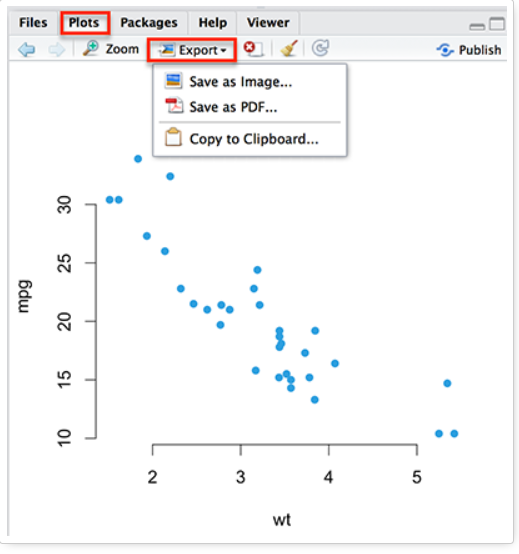
\includegraphics{1.PNG}
\caption{}
\end{figure}

\begin{Shaded}
\begin{Highlighting}[]
\CommentTok{#preference:http://www.sthda.com/english/wiki/r-base-graphs}
\end{Highlighting}
\end{Shaded}

\begin{enumerate}
\def\labelenumi{\arabic{enumi}.}
\setcounter{enumi}{1}
\tightlist
\item
  Using R codes:
\end{enumerate}

\begin{itemize}
\item
  \begin{enumerate}
  \def\labelenumi{\arabic{enumi}.}
  \tightlist
  \item
    Choose the format
  \end{enumerate}
\item
  \begin{enumerate}
  \def\labelenumi{\arabic{enumi}.}
  \setcounter{enumi}{1}
  \tightlist
  \item
    Create the graphs
  \end{enumerate}
\item
  \begin{enumerate}
  \def\labelenumi{\arabic{enumi}.}
  \setcounter{enumi}{2}
  \tightlist
  \item
    Enter the dev.off() command
  \end{enumerate}
\end{itemize}

Example-\textgreater{}

\textbf{Note:} The file you save are in the current working directory.

The command to get directory is \texttt{getwd()}

\begin{Shaded}
\begin{Highlighting}[]
\CommentTok{# 1. Choose the format}
\KeywordTok{png}\NormalTok{(}\StringTok{"rplot.jpg"}\NormalTok{) }\CommentTok{#width = 25, height = "25"}

\CommentTok{# 2. Create the graphs}
\KeywordTok{plot}\NormalTok{(}\DataTypeTok{x =}\NormalTok{ mtcars}\OperatorTok{$}\NormalTok{wt, }\DataTypeTok{y =}\NormalTok{ mtcars}\OperatorTok{$}\NormalTok{mpg,}
     \DataTypeTok{pch =} \DecValTok{16}\NormalTok{, }\DataTypeTok{frame =} \OtherTok{FALSE}\NormalTok{,}
     \DataTypeTok{xlab =} \StringTok{"wt"}\NormalTok{, }\DataTypeTok{ylab =} \StringTok{"mpg"}\NormalTok{, }\DataTypeTok{col =} \StringTok{"#2E9FDF"}\NormalTok{)}

\CommentTok{# 3. Save the file with dev.off() command in directory}
\KeywordTok{dev.off}\NormalTok{()}
\end{Highlighting}
\end{Shaded}

\begin{verbatim}
## pdf 
##   2
\end{verbatim}

File formats for exporting plots are:

\begin{itemize}
\item
  \texttt{pdf("rplot.pdf")} : pdf file
\item
  \texttt{png("rplot.png")} : png file
\item
  \texttt{jpeg("rplot.jpg")} : jpeg file
\item
  \texttt{postscript("rplot.ps")}: postscript file
\item
  \texttt{bmp("rplot.bmp")} : bmp file
\item
  \texttt{win.metafile("rplot.wmf")} : windows metafile
\end{itemize}

\chapter{Standard graphical formatting in
R}\label{standard-graphical-formatting-in-r}

\textbf{Introduction plot() function: }

\texttt{plot()} function is generic function for plotting of R objects
in basic graphs.

\begin{itemize}
\item
  \texttt{par()} : the default settings (rows x columns) for plots.
\item
  \texttt{plot()} : the main function.
\item
  There are many other plot functions which are specific to some tasks
  such as \texttt{hist()}, \texttt{boxplot()}, etc. Most of them take
  the same arguments as the \texttt{plot()} function.
\end{itemize}

Formula:

\begin{quote}
plot(x, y, type=``p'')
\end{quote}

\begin{itemize}
\item
  \textbf{x} and \textbf{y}: the coordinates of points to plot
\item
  \texttt{type}:

  \begin{itemize}
  \item
    ``p'' for points,
  \item
    ``l'' for lines,
  \item
    ``b'' for both,
  \item
    ``c'' for the lines part alone of ``b'',
  \item
    ``o'' for both `overplotted',
  \item
    ``h'' for `histogram' like (or `high-density') vertical lines,
  \item
    ``s'' for stair steps,
  \item
    ``S'' for other steps, see `Details' below,
  \item
    ``n'' for no plotting.
  \end{itemize}
\end{itemize}

Example:

\begin{Shaded}
\begin{Highlighting}[]
\KeywordTok{par}\NormalTok{(}\DataTypeTok{mfrow=}\KeywordTok{c}\NormalTok{(}\DecValTok{3}\NormalTok{,}\DecValTok{3}\NormalTok{), }\DataTypeTok{mar=}\KeywordTok{c}\NormalTok{(}\DecValTok{3}\NormalTok{,}\DecValTok{3}\NormalTok{,}\DecValTok{1}\NormalTok{,}\DecValTok{0}\NormalTok{)}\OperatorTok{+}\NormalTok{.}\DecValTok{5}\NormalTok{, }\DataTypeTok{mgp=}\KeywordTok{c}\NormalTok{(}\FloatTok{1.6}\NormalTok{,.}\DecValTok{6}\NormalTok{,}\DecValTok{0}\NormalTok{))  }\CommentTok{# set up the graphics}
\NormalTok{x<-}\DecValTok{1}\OperatorTok{:}\DecValTok{5}\NormalTok{; y=x}\OperatorTok{*}\NormalTok{x}
\KeywordTok{plot}\NormalTok{(x, y, }\DataTypeTok{type=}\StringTok{"p"}\NormalTok{,}\DataTypeTok{col=}\StringTok{"blue"}\NormalTok{)}
\KeywordTok{plot}\NormalTok{(x, y, }\DataTypeTok{type=}\StringTok{"l"}\NormalTok{,}\DataTypeTok{col=}\StringTok{"bisque"}\NormalTok{)}
\KeywordTok{plot}\NormalTok{(x,y, }\DataTypeTok{type=}\StringTok{"b"}\NormalTok{,}\DataTypeTok{col=}\StringTok{"green"}\NormalTok{)}
\KeywordTok{plot}\NormalTok{(x, y, }\DataTypeTok{type=}\StringTok{"c"}\NormalTok{,}\DataTypeTok{col=}\StringTok{"red"}\NormalTok{)}
\KeywordTok{plot}\NormalTok{(x, y, }\DataTypeTok{type=}\StringTok{"o"}\NormalTok{,}\DataTypeTok{col=}\StringTok{"pink"}\NormalTok{)}
\KeywordTok{plot}\NormalTok{(x,y, }\DataTypeTok{type=}\StringTok{"h"}\NormalTok{,}\DataTypeTok{col=}\StringTok{"orange"}\NormalTok{)}
\KeywordTok{plot}\NormalTok{(x, y, }\DataTypeTok{type=}\StringTok{"s"}\NormalTok{,}\DataTypeTok{col=}\StringTok{"purple"}\NormalTok{)}
\KeywordTok{plot}\NormalTok{(x, y, }\DataTypeTok{type=}\StringTok{"S"}\NormalTok{,}\DataTypeTok{col=}\StringTok{"black"}\NormalTok{)}
\KeywordTok{plot}\NormalTok{(x,y, }\DataTypeTok{type=}\StringTok{"h"}\NormalTok{,}\DataTypeTok{col=}\StringTok{"blue"}\NormalTok{)}
\end{Highlighting}
\end{Shaded}

\includegraphics{bookdown-demo_files/figure-latex/unnamed-chunk-6-1.pdf}

For more color type used the sintaks \texttt{color()}

More info about \texttt{plot()} go to RDocumentation
\href{https://www.rdocumentation.org/packages/graphics/versions/3.5.1/topics/plot}{here}

\textbf{Titles: }

\begin{itemize}
\item
  \texttt{main="test"}: main titles
\item
  \texttt{sub="text"}: subtitle
\item
  \texttt{xlab="test"}: the name of the x axis
\item
  \texttt{ylab="test"}: the name of the y axis.
\end{itemize}

====Main title and axis labels====

\begin{Shaded}
\begin{Highlighting}[]
\NormalTok{x<-}\DecValTok{1}\OperatorTok{:}\DecValTok{5}\NormalTok{; y=x}\OperatorTok{*}\NormalTok{x}
\KeywordTok{plot}\NormalTok{(x, y, }\DataTypeTok{type=}\StringTok{"p"}\NormalTok{,}\DataTypeTok{col=}\StringTok{"blue"}\NormalTok{,}\DataTypeTok{main=}\StringTok{"Exponential"}\NormalTok{,}\DataTypeTok{sub=}\StringTok{"Example"}\NormalTok{,}\DataTypeTok{ylab=}\StringTok{"Y Axis"}\NormalTok{,}\DataTypeTok{xlab=}\StringTok{"X Axis"}\NormalTok{)}
\end{Highlighting}
\end{Shaded}

\includegraphics{bookdown-demo_files/figure-latex/unnamed-chunk-7-1.pdf}

====Title colors====

\begin{Shaded}
\begin{Highlighting}[]
\NormalTok{x<-}\DecValTok{1}\OperatorTok{:}\DecValTok{5}\NormalTok{; y=x}\OperatorTok{*}\NormalTok{x}
\KeywordTok{plot}\NormalTok{(x, y, }\DataTypeTok{type=}\StringTok{"p"}\NormalTok{,}\DataTypeTok{col=}\StringTok{"#B7F200"}\NormalTok{,}\DataTypeTok{main=}\StringTok{"Exponential"}\NormalTok{,}\DataTypeTok{sub=}\StringTok{"Example"}\NormalTok{,}\DataTypeTok{ylab=}\StringTok{"Y Axis"}\NormalTok{,}\DataTypeTok{xlab=}\StringTok{"X Axis"}\NormalTok{,}
     \DataTypeTok{col.main=}\StringTok{"red"}\NormalTok{, }\DataTypeTok{col.lab=}\StringTok{"blue"}\NormalTok{, }\DataTypeTok{col.sub=}\StringTok{"green"}\NormalTok{)}
\end{Highlighting}
\end{Shaded}

\includegraphics{bookdown-demo_files/figure-latex/unnamed-chunk-8-1.pdf}

====The font style====

The possible values for the font style are :

\texttt{1:\ normal\ text} \texttt{2:\ bold} \texttt{3:\ italic}
\texttt{4:\ bold\ and\ italic} \texttt{5\ :\ Symbol\ font}

\begin{Shaded}
\begin{Highlighting}[]
\NormalTok{x<-}\DecValTok{1}\OperatorTok{:}\DecValTok{5}\NormalTok{; y=x}\OperatorTok{*}\NormalTok{x}
\KeywordTok{plot}\NormalTok{(x, y, }\DataTypeTok{type=}\StringTok{"p"}\NormalTok{,}\DataTypeTok{col=}\StringTok{"blue"}\NormalTok{,}\DataTypeTok{main=}\StringTok{"Exponential"}\NormalTok{,}\DataTypeTok{sub=}\StringTok{"Example"}\NormalTok{,}\DataTypeTok{ylab=}\StringTok{"Y Axis"}\NormalTok{,}\DataTypeTok{xlab=}\StringTok{"X Axis"}\NormalTok{,}
     \DataTypeTok{font.main=}\DecValTok{1}\NormalTok{, }\DataTypeTok{font.lab=}\DecValTok{2}\NormalTok{, }\DataTypeTok{font.sub=}\DecValTok{3}
\NormalTok{     )}
\end{Highlighting}
\end{Shaded}

\includegraphics{bookdown-demo_files/figure-latex/unnamed-chunk-9-1.pdf}

====The font size====

\begin{Shaded}
\begin{Highlighting}[]
\NormalTok{x<-}\DecValTok{1}\OperatorTok{:}\DecValTok{5}\NormalTok{; y=x}\OperatorTok{*}\NormalTok{x}
\KeywordTok{plot}\NormalTok{(x, y, }\DataTypeTok{type=}\StringTok{"p"}\NormalTok{,}\DataTypeTok{col=}\StringTok{"blue"}\NormalTok{,}\DataTypeTok{main=}\StringTok{"Exponential"}\NormalTok{,}\DataTypeTok{sub=}\StringTok{"Example"}\NormalTok{,}\DataTypeTok{ylab=}\StringTok{"Y Axis"}\NormalTok{,}\DataTypeTok{xlab=}\StringTok{"X Axis"}\NormalTok{,}
     \DataTypeTok{cex.main=}\DecValTok{4}\NormalTok{, }\DataTypeTok{cex.lab=}\FloatTok{1.5}\NormalTok{, }\DataTypeTok{cex.sub=}\FloatTok{0.8}
\NormalTok{     )}
\end{Highlighting}
\end{Shaded}

\includegraphics{bookdown-demo_files/figure-latex/unnamed-chunk-10-1.pdf}

====Use the \texttt{title()} function====

\begin{Shaded}
\begin{Highlighting}[]
\NormalTok{x<-}\DecValTok{1}\OperatorTok{:}\DecValTok{5}\NormalTok{; y=x}\OperatorTok{*}\NormalTok{x}
\KeywordTok{plot}\NormalTok{(x, y, }\DataTypeTok{type=}\StringTok{"p"}\NormalTok{)}
\KeywordTok{title}\NormalTok{(}\DataTypeTok{main =} \StringTok{"Main title"}\NormalTok{, }\DataTypeTok{sub =} \StringTok{"Sub-title"}\NormalTok{,}
      \DataTypeTok{xlab =} \StringTok{"X"}\NormalTok{, }\DataTypeTok{ylab =} \StringTok{"Y"}\NormalTok{,}
      \DataTypeTok{cex.main =} \DecValTok{2}\NormalTok{,   }\DataTypeTok{font.main=} \DecValTok{4}\NormalTok{, }\DataTypeTok{col.main=} \StringTok{"red"}\NormalTok{,}
      \DataTypeTok{cex.sub =} \FloatTok{0.75}\NormalTok{, }\DataTypeTok{font.sub =} \DecValTok{2}\NormalTok{, }\DataTypeTok{col.sub =} \StringTok{"green"}\NormalTok{,}
      \DataTypeTok{col.lab =}\StringTok{"darkblue"}
\NormalTok{      )}
\end{Highlighting}
\end{Shaded}

\includegraphics{bookdown-demo_files/figure-latex/unnamed-chunk-11-1.pdf}

====Customize the titles using \texttt{par()} function====

\begin{Shaded}
\begin{Highlighting}[]
\KeywordTok{par}\NormalTok{(}
  \CommentTok{# Change the colors}
  \DataTypeTok{col.main=}\StringTok{"red"}\NormalTok{, }\DataTypeTok{col.lab=}\StringTok{"blue"}\NormalTok{, }\DataTypeTok{col.sub=}\StringTok{"black"}\NormalTok{,}
  \CommentTok{# Titles in italic and bold}
  \DataTypeTok{font.main=}\DecValTok{4}\NormalTok{, }\DataTypeTok{font.lab=}\DecValTok{4}\NormalTok{, }\DataTypeTok{font.sub=}\DecValTok{4}\NormalTok{,}
  \CommentTok{# Change font size}
  \DataTypeTok{cex.main=}\DecValTok{2}\NormalTok{, }\DataTypeTok{cex.lab=}\FloatTok{1.7}\NormalTok{, }\DataTypeTok{cex.sub=}\FloatTok{1.2}
\NormalTok{  )}
\KeywordTok{plot}\NormalTok{(x, y, }\DataTypeTok{type=}\StringTok{"p"}\NormalTok{,}
     \DataTypeTok{main=}\StringTok{"TMain title"}\NormalTok{,}
        \DataTypeTok{xlab=}\StringTok{"X axis"}\NormalTok{,}
        \DataTypeTok{ylab=}\StringTok{"Y axis"}\NormalTok{,}
        \DataTypeTok{sub=}\StringTok{"Sub title"}
\NormalTok{     )}
\end{Highlighting}
\end{Shaded}

\includegraphics{bookdown-demo_files/figure-latex/unnamed-chunk-12-1.pdf}

\textbf{Legend: }

\texttt{legend()}: the position can be ``bottomleft'', ``bottomright'',
``topleft'', ``topright'' or exact coordinates.

====R legend function====

Formula:

\begin{quote}
legend(x, y=NULL, legend, fill, col, bg)
\end{quote}

Example:

\begin{Shaded}
\begin{Highlighting}[]
\CommentTok{# Generate example data}
\NormalTok{x<-}\DecValTok{1}\OperatorTok{:}\DecValTok{5}\NormalTok{; y1=x}\OperatorTok{*}\NormalTok{x; y2=}\DecValTok{3}\OperatorTok{*}\NormalTok{y1}
\KeywordTok{plot}\NormalTok{(x, y1, }\DataTypeTok{type=}\StringTok{"b"}\NormalTok{, }\DataTypeTok{pch=}\DecValTok{19}\NormalTok{, }\DataTypeTok{col=}\StringTok{"#FFD900"}\NormalTok{, }\DataTypeTok{xlab=}\StringTok{"x"}\NormalTok{, }\DataTypeTok{ylab=}\StringTok{"y"}\NormalTok{)}
\CommentTok{# Add a line}
\KeywordTok{lines}\NormalTok{(x, y2, }\DataTypeTok{pch=}\DecValTok{18}\NormalTok{, }\DataTypeTok{col=}\StringTok{"#8C6DD7"}\NormalTok{, }\DataTypeTok{type=}\StringTok{"b"}\NormalTok{, }\DataTypeTok{lty=}\DecValTok{2}\NormalTok{)}
\CommentTok{# Add a legend}
\KeywordTok{legend}\NormalTok{(}\DecValTok{1}\NormalTok{, }\DecValTok{20}\NormalTok{, }\DataTypeTok{legend=}\KeywordTok{c}\NormalTok{(}\StringTok{"Line 1"}\NormalTok{, }\StringTok{"Line 2"}\NormalTok{),}
       \DataTypeTok{col=}\KeywordTok{c}\NormalTok{(}\StringTok{"#FFD900"}\NormalTok{, }\StringTok{"#8C6DD7"}\NormalTok{), }\DataTypeTok{lty=}\DecValTok{1}\OperatorTok{:}\DecValTok{2}\NormalTok{, }\DataTypeTok{cex=}\FloatTok{0.8}\NormalTok{)}
\end{Highlighting}
\end{Shaded}

\includegraphics{bookdown-demo_files/figure-latex/unnamed-chunk-13-1.pdf}

Create R function to avoid repeating graphs code:

\begin{Shaded}
\begin{Highlighting}[]
\CommentTok{# Generate example data}
\NormalTok{make_plot<-}\ControlFlowTok{function}\NormalTok{()\{}
\NormalTok{x<-}\DecValTok{1}\OperatorTok{:}\DecValTok{5}\NormalTok{; y1=x}\OperatorTok{*}\NormalTok{x; y2=}\DecValTok{3}\OperatorTok{*}\NormalTok{y1}
\KeywordTok{plot}\NormalTok{(x, y1, }\DataTypeTok{type=}\StringTok{"b"}\NormalTok{, }\DataTypeTok{pch=}\DecValTok{19}\NormalTok{, }\DataTypeTok{col=}\StringTok{"red"}\NormalTok{, }\DataTypeTok{xlab=}\StringTok{"x"}\NormalTok{, }\DataTypeTok{ylab=}\StringTok{"y"}\NormalTok{)}
\CommentTok{# Add a line}
\KeywordTok{lines}\NormalTok{(x, y2, }\DataTypeTok{pch=}\DecValTok{18}\NormalTok{, }\DataTypeTok{col=}\StringTok{"blue"}\NormalTok{, }\DataTypeTok{type=}\StringTok{"b"}\NormalTok{, }\DataTypeTok{lty=}\DecValTok{2}\NormalTok{)}
\CommentTok{# Add a legend}
\KeywordTok{legend}\NormalTok{(}\DecValTok{1}\NormalTok{, }\DecValTok{20}\NormalTok{, }\DataTypeTok{legend=}\KeywordTok{c}\NormalTok{(}\StringTok{"Line 1"}\NormalTok{, }\StringTok{"Line 2"}\NormalTok{),}
       \DataTypeTok{col=}\KeywordTok{c}\NormalTok{(}\StringTok{"red"}\NormalTok{, }\StringTok{"blue"}\NormalTok{), }\DataTypeTok{lty=}\DecValTok{1}\OperatorTok{:}\DecValTok{2}\NormalTok{, }\DataTypeTok{cex=}\FloatTok{0.8}\NormalTok{)}
\NormalTok{\}}
\end{Highlighting}
\end{Shaded}

\begin{Shaded}
\begin{Highlighting}[]
\KeywordTok{make_plot}\NormalTok{()}
\end{Highlighting}
\end{Shaded}

\includegraphics{bookdown-demo_files/figure-latex/unnamed-chunk-15-1.pdf}

====Title, text font and background color of the legend box====

\begin{itemize}
\tightlist
\item
  title: The title of the legend
\item
  text.font: an integer specifying the font style of the legend text;
  possible values are :

  \begin{itemize}
  \tightlist
  \item
    1: normal
  \item
    2: bold
  \item
    3: italic
  \item
    4: bold and italic
  \item
    bg: background color of the legend box
  \end{itemize}
\end{itemize}

\begin{Shaded}
\begin{Highlighting}[]
\KeywordTok{make_plot}\NormalTok{()}

\CommentTok{# Add a legend to the plot}
\KeywordTok{legend}\NormalTok{(}\DecValTok{1}\NormalTok{,}\DecValTok{20}\NormalTok{, }\DataTypeTok{legend=}\KeywordTok{c}\NormalTok{(}\StringTok{"Line 1"}\NormalTok{, }\StringTok{"Line 2"}\NormalTok{),}
       \DataTypeTok{col=}\KeywordTok{c}\NormalTok{(}\StringTok{"red"}\NormalTok{, }\StringTok{"blue"}\NormalTok{), }\DataTypeTok{lty=}\DecValTok{1}\OperatorTok{:}\DecValTok{2}\NormalTok{, }\DataTypeTok{cex=}\FloatTok{0.8}\NormalTok{,}
       \DataTypeTok{title=}\StringTok{"Line types"}\NormalTok{, }\DataTypeTok{text.font=}\DecValTok{4}\NormalTok{, }\DataTypeTok{bg=}\StringTok{"lightblue"}\NormalTok{)}
\end{Highlighting}
\end{Shaded}

\includegraphics{bookdown-demo_files/figure-latex/unnamed-chunk-16-1.pdf}

====Border of the legend box====

\begin{itemize}
\item
  box.lty: modify the line type
\item
  box.lwd: modify the width
\item
  box.col: modify the color
\end{itemize}

\begin{Shaded}
\begin{Highlighting}[]
\KeywordTok{par}\NormalTok{(}\DataTypeTok{mfrow=}\KeywordTok{c}\NormalTok{(}\DecValTok{2}\NormalTok{,}\DecValTok{1}\NormalTok{), }\DataTypeTok{mar=}\KeywordTok{c}\NormalTok{(}\DecValTok{3}\NormalTok{,}\DecValTok{3}\NormalTok{,}\DecValTok{1}\NormalTok{,}\DecValTok{0}\NormalTok{)}\OperatorTok{+}\NormalTok{.}\DecValTok{5}\NormalTok{, }\DataTypeTok{mgp=}\KeywordTok{c}\NormalTok{(}\FloatTok{1.6}\NormalTok{,.}\DecValTok{6}\NormalTok{,}\DecValTok{0}\NormalTok{))  }\CommentTok{# set up the graphics}
\CommentTok{# Remove legend border using box.lty = 0}
\KeywordTok{make_plot}\NormalTok{()}
\KeywordTok{legend}\NormalTok{(}\DecValTok{1}\NormalTok{,}\DecValTok{20}\NormalTok{, }\DataTypeTok{legend=}\KeywordTok{c}\NormalTok{(}\StringTok{"Line 1"}\NormalTok{, }\StringTok{"Line 2"}\NormalTok{),}
       \DataTypeTok{col=}\KeywordTok{c}\NormalTok{(}\StringTok{"red"}\NormalTok{, }\StringTok{"blue"}\NormalTok{), }\DataTypeTok{lty=}\DecValTok{1}\OperatorTok{:}\DecValTok{2}\NormalTok{, }\DataTypeTok{cex=}\FloatTok{0.8}\NormalTok{,}
       \DataTypeTok{box.lty=}\DecValTok{0}\NormalTok{)}
\CommentTok{# Change the border}
\KeywordTok{make_plot}\NormalTok{()}
\KeywordTok{legend}\NormalTok{(}\DecValTok{1}\NormalTok{,}\DecValTok{20}\NormalTok{, }\DataTypeTok{legend=}\KeywordTok{c}\NormalTok{(}\StringTok{"Line 1"}\NormalTok{, }\StringTok{"Line 2"}\NormalTok{),}
       \DataTypeTok{col=}\KeywordTok{c}\NormalTok{(}\StringTok{"red"}\NormalTok{, }\StringTok{"blue"}\NormalTok{), }\DataTypeTok{lty=}\DecValTok{1}\OperatorTok{:}\DecValTok{2}\NormalTok{, }\DataTypeTok{cex=}\FloatTok{0.8}\NormalTok{,}
       \DataTypeTok{box.lty=}\DecValTok{2}\NormalTok{, }\DataTypeTok{box.lwd=}\DecValTok{2}\NormalTok{, }\DataTypeTok{box.col=}\StringTok{"green"}\NormalTok{)}
\end{Highlighting}
\end{Shaded}

\includegraphics{bookdown-demo_files/figure-latex/unnamed-chunk-17-1.pdf}

====The legend position by keywords====

Using the following keywords : ``bottomright'', ``bottom'',
``bottomleft'', ``left'', ``topleft'', ``top'', ``topright'', ``right''
and ``center''.

\begin{figure}
\centering
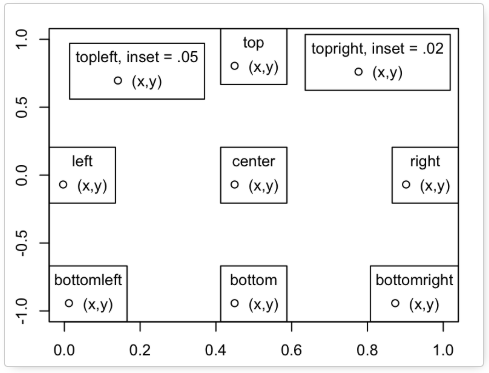
\includegraphics{2.PNG}
\caption{}
\end{figure}

\begin{Shaded}
\begin{Highlighting}[]
\KeywordTok{par}\NormalTok{(}\DataTypeTok{mfrow=}\KeywordTok{c}\NormalTok{(}\DecValTok{2}\NormalTok{,}\DecValTok{1}\NormalTok{), }\DataTypeTok{mar=}\KeywordTok{c}\NormalTok{(}\DecValTok{3}\NormalTok{,}\DecValTok{3}\NormalTok{,}\DecValTok{1}\NormalTok{,}\DecValTok{0}\NormalTok{)}\OperatorTok{+}\NormalTok{.}\DecValTok{5}\NormalTok{, }\DataTypeTok{mgp=}\KeywordTok{c}\NormalTok{(}\FloatTok{1.6}\NormalTok{,.}\DecValTok{6}\NormalTok{,}\DecValTok{0}\NormalTok{))  }\CommentTok{# set up the graphics}
\CommentTok{# Remove legend border using box.lty = 0}
\KeywordTok{make_plot}\NormalTok{()}
\KeywordTok{legend}\NormalTok{(}\StringTok{"center"}\NormalTok{, }\DataTypeTok{legend=}\KeywordTok{c}\NormalTok{(}\StringTok{"Line 1"}\NormalTok{, }\StringTok{"Line 2"}\NormalTok{),}
       \DataTypeTok{col=}\KeywordTok{c}\NormalTok{(}\StringTok{"red"}\NormalTok{, }\StringTok{"blue"}\NormalTok{),}\DataTypeTok{box.lty=}\DecValTok{0}\NormalTok{)}
\KeywordTok{make_plot}\NormalTok{()}
\KeywordTok{legend}\NormalTok{(}\StringTok{"topright"}\NormalTok{, }\DataTypeTok{legend=}\KeywordTok{c}\NormalTok{(}\StringTok{"Line 1"}\NormalTok{, }\StringTok{"Line 2"}\NormalTok{),}
       \DataTypeTok{col=}\KeywordTok{c}\NormalTok{(}\StringTok{"red"}\NormalTok{, }\StringTok{"blue"}\NormalTok{),}
       \DataTypeTok{box.lty=}\DecValTok{0}\NormalTok{)}
\end{Highlighting}
\end{Shaded}

\includegraphics{bookdown-demo_files/figure-latex/unnamed-chunk-18-1.pdf}

\textbf{Text: }

\texttt{text()} and \texttt{mtext()} R functions can be used To add a
text to a plot.

====Texts within the graph====

Formula:

\begin{quote}
text(x, y, labels)
\end{quote}

Example:

\begin{Shaded}
\begin{Highlighting}[]
\NormalTok{d<-}\KeywordTok{head}\NormalTok{(mtcars)}
\KeywordTok{plot}\NormalTok{(d[,}\StringTok{'wt'}\NormalTok{], d[,}\StringTok{'mpg'}\NormalTok{], }
     \DataTypeTok{main=}\StringTok{"Milage vs. Car Weight}\CharTok{\textbackslash{}n}\StringTok{~~~~~~~~~~~~~~~~~~~"}\NormalTok{,}
      \DataTypeTok{xlab=}\StringTok{"Weight"}\NormalTok{, }\DataTypeTok{ylab=}\StringTok{"Miles/(US) gallon"}\NormalTok{,}
      \DataTypeTok{pch=}\DecValTok{19}\NormalTok{, }\DataTypeTok{col=}\StringTok{"darkgreen"}\NormalTok{)}
\KeywordTok{text}\NormalTok{(d[,}\StringTok{'wt'}\NormalTok{], d[,}\StringTok{'mpg'}\NormalTok{],  }\KeywordTok{row.names}\NormalTok{(d),}
     \DataTypeTok{cex=}\FloatTok{0.85}\NormalTok{, }\DataTypeTok{pos=}\DecValTok{2}\NormalTok{,}\DataTypeTok{col=}\StringTok{"red"}\NormalTok{)}
\end{Highlighting}
\end{Shaded}

\includegraphics{bookdown-demo_files/figure-latex/unnamed-chunk-19-1.pdf}

====Text in the margins of the graph====

\begin{itemize}
\tightlist
\item
  text : the text to be written
\item
  side : an integer specifying the side of the plot; Possible values are
  :
\item
  1: bottom
\item
  2: left
\item
  3: top
\item
  4: right
\end{itemize}

\begin{Shaded}
\begin{Highlighting}[]
\KeywordTok{plot}\NormalTok{(}\DecValTok{1}\OperatorTok{:}\DecValTok{7}\NormalTok{, }\DecValTok{1}\OperatorTok{:}\DecValTok{7}\NormalTok{, }
     \DataTypeTok{main=}\StringTok{"mtext(...) examples"}\NormalTok{,}\DataTypeTok{col=}\StringTok{"blue"}\NormalTok{)}
\KeywordTok{mtext}\NormalTok{(}\StringTok{"Magic function"}\NormalTok{, }\DataTypeTok{side=}\DecValTok{4}\NormalTok{)}
\end{Highlighting}
\end{Shaded}

\includegraphics{bookdown-demo_files/figure-latex/unnamed-chunk-20-1.pdf}

====Mathematical annotation within the graph====

Example:

\begin{Shaded}
\begin{Highlighting}[]
\KeywordTok{plot}\NormalTok{(}\DecValTok{1}\OperatorTok{:}\DecValTok{7}\NormalTok{, }\DecValTok{1}\OperatorTok{:}\DecValTok{7}\NormalTok{, }
     \DataTypeTok{main=}\StringTok{"text(...) examples"}\NormalTok{,}\DataTypeTok{col=}\StringTok{"black"}\NormalTok{)}
\KeywordTok{text}\NormalTok{(}\DecValTok{2}\NormalTok{, }\DecValTok{4}\NormalTok{, }\KeywordTok{expression}\NormalTok{(}\KeywordTok{hat}\NormalTok{(beta) }\OperatorTok{==}\StringTok{ }\NormalTok{(X}\OperatorTok{^}\NormalTok{t }\OperatorTok{*}\StringTok{ }\NormalTok{X)}\OperatorTok{^}\NormalTok{\{}\OperatorTok{-}\DecValTok{1}\NormalTok{\} }\OperatorTok{*}\StringTok{ }\NormalTok{X}\OperatorTok{^}\NormalTok{t }\OperatorTok{*}\StringTok{ }\NormalTok{y))}
\KeywordTok{text}\NormalTok{(}\DecValTok{2}\NormalTok{, }\DecValTok{6}\NormalTok{, }\KeywordTok{expression}\NormalTok{(}\KeywordTok{bar}\NormalTok{(x) }\OperatorTok{==}\StringTok{ }\KeywordTok{sum}\NormalTok{(}\KeywordTok{frac}\NormalTok{(x[i], n), i}\OperatorTok{==}\DecValTok{1}\NormalTok{, n)))}
\end{Highlighting}
\end{Shaded}

\includegraphics{bookdown-demo_files/figure-latex/unnamed-chunk-21-1.pdf}

\textbf{Types of Plot: }

An option for plot types can be:

\texttt{type}: * ``p'' for points,

\begin{verbatim}
  * "l" for lines,

  * "b" for both,

  * "c" for the lines part alone of "b",

  * "o" for both 'overplotted',

  * "h" for 'histogram' like (or 'high-density') vertical lines,

  * "s" for stair steps,

  * "S" for other steps, see 'Details' below,

  * "n" for no plotting.
\end{verbatim}

\begin{Shaded}
\begin{Highlighting}[]
\NormalTok{x <-}\StringTok{ }\KeywordTok{rnorm}\NormalTok{(}\DecValTok{100}\NormalTok{) }
\KeywordTok{par}\NormalTok{(}\DataTypeTok{mfrow =} \KeywordTok{c}\NormalTok{(}\DecValTok{2}\NormalTok{,}\DecValTok{2}\NormalTok{))}
\KeywordTok{plot}\NormalTok{(x, }\DataTypeTok{type =} \StringTok{"p"}\NormalTok{, }\DataTypeTok{main =} \StringTok{"points"}\NormalTok{, }\DataTypeTok{ylab =} \StringTok{""}\NormalTok{, }\DataTypeTok{xlab =} \StringTok{""}\NormalTok{,}\DataTypeTok{col=}\StringTok{"red"}\NormalTok{)}
\KeywordTok{plot}\NormalTok{(x, }\DataTypeTok{type =} \StringTok{"o"}\NormalTok{, }\DataTypeTok{main =} \StringTok{"overplotted"}\NormalTok{, }\DataTypeTok{ylab =} \StringTok{""}\NormalTok{, }\DataTypeTok{xlab =} \StringTok{""}\NormalTok{,}\DataTypeTok{col=}\StringTok{"green"}\NormalTok{)}
\KeywordTok{plot}\NormalTok{(x, }\DataTypeTok{type =} \StringTok{"h"}\NormalTok{, }\DataTypeTok{main =} \StringTok{"histogram"}\NormalTok{, }\DataTypeTok{ylab =} \StringTok{""}\NormalTok{, }\DataTypeTok{xlab =} \StringTok{""}\NormalTok{,}\DataTypeTok{col=}\StringTok{"blue"}\NormalTok{)}
\KeywordTok{plot}\NormalTok{(x, }\DataTypeTok{type =} \StringTok{"S"}\NormalTok{, }\DataTypeTok{main =} \StringTok{"steps"}\NormalTok{, }\DataTypeTok{ylab =} \StringTok{""}\NormalTok{, }\DataTypeTok{xlab =} \StringTok{""}\NormalTok{,}\DataTypeTok{col=}\StringTok{"orange"}\NormalTok{)}
\end{Highlighting}
\end{Shaded}

\includegraphics{bookdown-demo_files/figure-latex/unnamed-chunk-22-1.pdf}

\textbf{Axis: }

====Add an axis to a plot====

Formula:

\begin{quote}
axis(side, at=NULL, labels=TRUE)
\end{quote}

Side :

\begin{itemize}
\item
  1: below
\item
  2: left
\item
  3: above
\item
  4: right
\item
  at: The position
\item
  labels: Texts for tick-mark labels.
\end{itemize}

Example :

\begin{Shaded}
\begin{Highlighting}[]
\KeywordTok{par}\NormalTok{(}\DataTypeTok{mfrow=}\KeywordTok{c}\NormalTok{(}\DecValTok{3}\NormalTok{,}\DecValTok{1}\NormalTok{), }\DataTypeTok{mar=}\KeywordTok{c}\NormalTok{(}\DecValTok{3}\NormalTok{,}\DecValTok{3}\NormalTok{,}\DecValTok{1}\NormalTok{,}\DecValTok{0}\NormalTok{)}\OperatorTok{+}\NormalTok{.}\DecValTok{5}\NormalTok{, }\DataTypeTok{mgp=}\KeywordTok{c}\NormalTok{(}\FloatTok{1.6}\NormalTok{,.}\DecValTok{6}\NormalTok{,}\DecValTok{0}\NormalTok{))  }\CommentTok{# set up the graphics}
\NormalTok{x<-}\DecValTok{1}\OperatorTok{:}\DecValTok{3}\NormalTok{; y=x}\OperatorTok{*}\NormalTok{x}
\CommentTok{# Example 1}
\KeywordTok{plot}\NormalTok{(x, y, }\DataTypeTok{axes =} \OtherTok{FALSE}\NormalTok{)}
\KeywordTok{axis}\NormalTok{(}\DataTypeTok{side=}\DecValTok{1}\NormalTok{, }\DataTypeTok{at =} \DecValTok{1}\OperatorTok{:}\DecValTok{3}\NormalTok{, }\DataTypeTok{labels=}\NormalTok{LETTERS[}\DecValTok{1}\OperatorTok{:}\DecValTok{3}\NormalTok{])}
\KeywordTok{axis}\NormalTok{(}\DecValTok{2}\NormalTok{)}
\CommentTok{# Example 2}
\KeywordTok{plot}\NormalTok{(x, y, }\DataTypeTok{axes =} \OtherTok{FALSE}\NormalTok{)}
\KeywordTok{axis}\NormalTok{(}\DataTypeTok{side=}\DecValTok{1}\NormalTok{, }\DataTypeTok{at=}\DecValTok{1}\OperatorTok{:}\DecValTok{3}\NormalTok{, }\DataTypeTok{labels=}\NormalTok{LETTERS[}\DecValTok{1}\OperatorTok{:}\DecValTok{3}\NormalTok{])}
\KeywordTok{axis}\NormalTok{(}\DecValTok{2}\NormalTok{)}
\KeywordTok{box}\NormalTok{() }\CommentTok{#- To make it look like "usual" plot}
\CommentTok{#Example3:}
\KeywordTok{plot}\NormalTok{(x, y, }\DataTypeTok{pch=}\DecValTok{18}\NormalTok{, }\DataTypeTok{col=}\StringTok{"red"}\NormalTok{, }\DataTypeTok{type=}\StringTok{"b"}\NormalTok{,}
     \DataTypeTok{frame=}\OtherTok{FALSE}\NormalTok{, }\DataTypeTok{xaxt=}\StringTok{"n"}\NormalTok{) }\CommentTok{# Remove x axis}
\KeywordTok{axis}\NormalTok{(}\DecValTok{1}\NormalTok{, }\DecValTok{1}\OperatorTok{:}\DecValTok{4}\NormalTok{, LETTERS[}\DecValTok{1}\OperatorTok{:}\DecValTok{4}\NormalTok{], }\DataTypeTok{col.axis=}\StringTok{"blue"}\NormalTok{)}
\KeywordTok{axis}\NormalTok{(}\DecValTok{3}\NormalTok{, }\DataTypeTok{col =} \StringTok{"darkgreen"}\NormalTok{, }\DataTypeTok{lty =} \DecValTok{2}\NormalTok{, }\DataTypeTok{lwd =} \FloatTok{0.5}\NormalTok{)}
\KeywordTok{axis}\NormalTok{(}\DecValTok{4}\NormalTok{, }\DataTypeTok{col =} \StringTok{"violet"}\NormalTok{, }\DataTypeTok{col.axis =} \StringTok{"dark violet"}\NormalTok{, }\DataTypeTok{lwd =} \DecValTok{2}\NormalTok{)}
\end{Highlighting}
\end{Shaded}

\includegraphics{bookdown-demo_files/figure-latex/unnamed-chunk-23-1.pdf}

====Axis scale====

\begin{itemize}
\item
  xlim: the limit of x axis; format : xlim = c(min, max)
\item
  ylim: the limit of y axis; format: ylim = c(min, max)
\end{itemize}

Transformation to log scale:

\begin{itemize}
\item
  log = ``x''
\item
  log = ``y''
\item
  log = ``xy''*
\end{itemize}

Example:

\begin{Shaded}
\begin{Highlighting}[]
\KeywordTok{par}\NormalTok{(}\DataTypeTok{mfrow=}\KeywordTok{c}\NormalTok{(}\DecValTok{3}\NormalTok{,}\DecValTok{1}\NormalTok{), }\DataTypeTok{mar=}\KeywordTok{c}\NormalTok{(}\DecValTok{3}\NormalTok{,}\DecValTok{3}\NormalTok{,}\DecValTok{1}\NormalTok{,}\DecValTok{0}\NormalTok{)}\OperatorTok{+}\NormalTok{.}\DecValTok{5}\NormalTok{, }\DataTypeTok{mgp=}\KeywordTok{c}\NormalTok{(}\FloatTok{1.6}\NormalTok{,.}\DecValTok{6}\NormalTok{,}\DecValTok{0}\NormalTok{))  }\CommentTok{# set up the graphics}
\NormalTok{x<-}\DecValTok{1}\OperatorTok{:}\DecValTok{20}\NormalTok{; y=x}\OperatorTok{*}\NormalTok{x}
\CommentTok{# Simple graph}
\KeywordTok{plot}\NormalTok{(x, y,}\DataTypeTok{col=}\StringTok{"blue"}\NormalTok{)}
\CommentTok{# Enlarge the scale}
\KeywordTok{plot}\NormalTok{(x, y, }\DataTypeTok{xlim=}\KeywordTok{c}\NormalTok{(}\DecValTok{1}\NormalTok{,}\DecValTok{15}\NormalTok{), }\DataTypeTok{ylim=}\KeywordTok{c}\NormalTok{(}\DecValTok{1}\NormalTok{,}\DecValTok{150}\NormalTok{),}\DataTypeTok{col=}\StringTok{"blue"}\NormalTok{)}
\CommentTok{# Log scale}
\KeywordTok{plot}\NormalTok{(x, y, }\DataTypeTok{log=}\StringTok{"y"}\NormalTok{,}\DataTypeTok{col=}\StringTok{"blue"}\NormalTok{)}
\end{Highlighting}
\end{Shaded}

\includegraphics{bookdown-demo_files/figure-latex/unnamed-chunk-24-1.pdf}

====Axes fonts====

Remove them with \texttt{axes=FALSE}:

\begin{Shaded}
\begin{Highlighting}[]
\KeywordTok{par}\NormalTok{(}\DataTypeTok{mfrow=}\KeywordTok{c}\NormalTok{(}\DecValTok{2}\NormalTok{,}\DecValTok{1}\NormalTok{), }\DataTypeTok{mar=}\KeywordTok{c}\NormalTok{(}\DecValTok{3}\NormalTok{,}\DecValTok{3}\NormalTok{,}\DecValTok{1}\NormalTok{,}\DecValTok{0}\NormalTok{)}\OperatorTok{+}\NormalTok{.}\DecValTok{5}\NormalTok{, }\DataTypeTok{mgp=}\KeywordTok{c}\NormalTok{(}\FloatTok{1.6}\NormalTok{,.}\DecValTok{6}\NormalTok{,}\DecValTok{0}\NormalTok{))  }\CommentTok{# set up the graphics}
\NormalTok{x1<-}\DecValTok{1}\OperatorTok{:}\DecValTok{10}
\NormalTok{x2<-}\DecValTok{11}\OperatorTok{:}\DecValTok{20}
\KeywordTok{plot}\NormalTok{(x1,x2,}\DataTypeTok{axes=}\OtherTok{FALSE}\NormalTok{)}
\KeywordTok{plot}\NormalTok{(x1,x2,}\DataTypeTok{axes=}\OtherTok{FALSE}\NormalTok{)}
\KeywordTok{axis}\NormalTok{(}\DecValTok{1}\NormalTok{,}\DataTypeTok{col=}\StringTok{"red"}\NormalTok{,}\DataTypeTok{col.axis=}\StringTok{"blue"}\NormalTok{,}\DataTypeTok{font.axis=}\DecValTok{3}\NormalTok{)}
\KeywordTok{axis}\NormalTok{(}\DecValTok{2}\NormalTok{,}\DataTypeTok{col=}\StringTok{"red"}\NormalTok{,}\DataTypeTok{col.axis=}\StringTok{"blue"}\NormalTok{,}\DataTypeTok{font.axis=}\DecValTok{2}\NormalTok{,}\DataTypeTok{las=}\DecValTok{2}\NormalTok{)}
\end{Highlighting}
\end{Shaded}

\includegraphics{bookdown-demo_files/figure-latex/unnamed-chunk-25-1.pdf}

====Axes positions====

Use \texttt{las} function to specified the style of axis labels:

\begin{itemize}
\item
  0 : always parallel to the axis {[}default{]}
\item
  1 : always horizontal
\item
  2 : always perpendicular to the axis
\item
  3 : always vertical
\end{itemize}

\begin{Shaded}
\begin{Highlighting}[]
\NormalTok{x1 <-}\StringTok{ }\KeywordTok{rnorm}\NormalTok{(}\DecValTok{150}\NormalTok{)}
\KeywordTok{par}\NormalTok{(}\DataTypeTok{mfrow =} \KeywordTok{c}\NormalTok{(}\DecValTok{2}\NormalTok{,}\DecValTok{2}\NormalTok{))}
\KeywordTok{plot}\NormalTok{(x1, }\DataTypeTok{las =} \DecValTok{0}\NormalTok{, }\DataTypeTok{main =} \StringTok{"las = 0"}\NormalTok{, }\DataTypeTok{sub =} \StringTok{"always parallel to the axis"}\NormalTok{, }\DataTypeTok{xlab =} \StringTok{""}\NormalTok{, }\DataTypeTok{ylab =} \StringTok{""}\NormalTok{,}\DataTypeTok{col=}\StringTok{"blue"}\NormalTok{)}
\KeywordTok{plot}\NormalTok{(x1, }\DataTypeTok{las =} \DecValTok{1}\NormalTok{, }\DataTypeTok{main =} \StringTok{"las = 1"}\NormalTok{, }\DataTypeTok{sub =} \StringTok{"always horizontal"}\NormalTok{, }\DataTypeTok{xlab =} \StringTok{""}\NormalTok{, }\DataTypeTok{ylab =} \StringTok{""}\NormalTok{,}\DataTypeTok{col=}\StringTok{"blue"}\NormalTok{) }
\KeywordTok{plot}\NormalTok{(x1, }\DataTypeTok{las =} \DecValTok{2}\NormalTok{, }\DataTypeTok{main =} \StringTok{"las = 2"}\NormalTok{, }\DataTypeTok{sub =} \StringTok{"always perpendicular to the axis"}\NormalTok{, }\DataTypeTok{xlab =} \StringTok{""}\NormalTok{, }\DataTypeTok{ylab =} \StringTok{""}\NormalTok{,}\DataTypeTok{col=}\StringTok{"blue"}\NormalTok{)}
\KeywordTok{plot}\NormalTok{(x1, }\DataTypeTok{las =} \DecValTok{3}\NormalTok{, }\DataTypeTok{main =} \StringTok{"las = 3"}\NormalTok{, }\DataTypeTok{sub =} \StringTok{"always vertical"}\NormalTok{, }\DataTypeTok{xlab =} \StringTok{""}\NormalTok{, }\DataTypeTok{ylab =} \StringTok{""}\NormalTok{,}\DataTypeTok{col=}\StringTok{"blue"}\NormalTok{)}
\end{Highlighting}
\end{Shaded}

\includegraphics{bookdown-demo_files/figure-latex/unnamed-chunk-26-1.pdf}

\textbf{Margins \texttt{par()}: }

Formula:

\begin{quote}
par(mfrow=c(2,1), mar=c(3,3,1,0)+.5, mgp=c(1.6,.6,0)) \# set up the
graphics
\end{quote}

See \texttt{?par} to learn more about the topic.

\textbf{Colors: }

Use by name (e.g col = ``red'') or as a hexadecimal RGB triplet (such as
col = ``\#FFCC00'').

====Default color in R====

\begin{Shaded}
\begin{Highlighting}[]
\KeywordTok{colors}\NormalTok{() }\CommentTok{# list the r colors}
\end{Highlighting}
\end{Shaded}

\begin{verbatim}
##   [1] "white"                "aliceblue"            "antiquewhite"        
##   [4] "antiquewhite1"        "antiquewhite2"        "antiquewhite3"       
##   [7] "antiquewhite4"        "aquamarine"           "aquamarine1"         
##  [10] "aquamarine2"          "aquamarine3"          "aquamarine4"         
##  [13] "azure"                "azure1"               "azure2"              
##  [16] "azure3"               "azure4"               "beige"               
##  [19] "bisque"               "bisque1"              "bisque2"             
##  [22] "bisque3"              "bisque4"              "black"               
##  [25] "blanchedalmond"       "blue"                 "blue1"               
##  [28] "blue2"                "blue3"                "blue4"               
##  [31] "blueviolet"           "brown"                "brown1"              
##  [34] "brown2"               "brown3"               "brown4"              
##  [37] "burlywood"            "burlywood1"           "burlywood2"          
##  [40] "burlywood3"           "burlywood4"           "cadetblue"           
##  [43] "cadetblue1"           "cadetblue2"           "cadetblue3"          
##  [46] "cadetblue4"           "chartreuse"           "chartreuse1"         
##  [49] "chartreuse2"          "chartreuse3"          "chartreuse4"         
##  [52] "chocolate"            "chocolate1"           "chocolate2"          
##  [55] "chocolate3"           "chocolate4"           "coral"               
##  [58] "coral1"               "coral2"               "coral3"              
##  [61] "coral4"               "cornflowerblue"       "cornsilk"            
##  [64] "cornsilk1"            "cornsilk2"            "cornsilk3"           
##  [67] "cornsilk4"            "cyan"                 "cyan1"               
##  [70] "cyan2"                "cyan3"                "cyan4"               
##  [73] "darkblue"             "darkcyan"             "darkgoldenrod"       
##  [76] "darkgoldenrod1"       "darkgoldenrod2"       "darkgoldenrod3"      
##  [79] "darkgoldenrod4"       "darkgray"             "darkgreen"           
##  [82] "darkgrey"             "darkkhaki"            "darkmagenta"         
##  [85] "darkolivegreen"       "darkolivegreen1"      "darkolivegreen2"     
##  [88] "darkolivegreen3"      "darkolivegreen4"      "darkorange"          
##  [91] "darkorange1"          "darkorange2"          "darkorange3"         
##  [94] "darkorange4"          "darkorchid"           "darkorchid1"         
##  [97] "darkorchid2"          "darkorchid3"          "darkorchid4"         
## [100] "darkred"              "darksalmon"           "darkseagreen"        
## [103] "darkseagreen1"        "darkseagreen2"        "darkseagreen3"       
## [106] "darkseagreen4"        "darkslateblue"        "darkslategray"       
## [109] "darkslategray1"       "darkslategray2"       "darkslategray3"      
## [112] "darkslategray4"       "darkslategrey"        "darkturquoise"       
## [115] "darkviolet"           "deeppink"             "deeppink1"           
## [118] "deeppink2"            "deeppink3"            "deeppink4"           
## [121] "deepskyblue"          "deepskyblue1"         "deepskyblue2"        
## [124] "deepskyblue3"         "deepskyblue4"         "dimgray"             
## [127] "dimgrey"              "dodgerblue"           "dodgerblue1"         
## [130] "dodgerblue2"          "dodgerblue3"          "dodgerblue4"         
## [133] "firebrick"            "firebrick1"           "firebrick2"          
## [136] "firebrick3"           "firebrick4"           "floralwhite"         
## [139] "forestgreen"          "gainsboro"            "ghostwhite"          
## [142] "gold"                 "gold1"                "gold2"               
## [145] "gold3"                "gold4"                "goldenrod"           
## [148] "goldenrod1"           "goldenrod2"           "goldenrod3"          
## [151] "goldenrod4"           "gray"                 "gray0"               
## [154] "gray1"                "gray2"                "gray3"               
## [157] "gray4"                "gray5"                "gray6"               
## [160] "gray7"                "gray8"                "gray9"               
## [163] "gray10"               "gray11"               "gray12"              
## [166] "gray13"               "gray14"               "gray15"              
## [169] "gray16"               "gray17"               "gray18"              
## [172] "gray19"               "gray20"               "gray21"              
## [175] "gray22"               "gray23"               "gray24"              
## [178] "gray25"               "gray26"               "gray27"              
## [181] "gray28"               "gray29"               "gray30"              
## [184] "gray31"               "gray32"               "gray33"              
## [187] "gray34"               "gray35"               "gray36"              
## [190] "gray37"               "gray38"               "gray39"              
## [193] "gray40"               "gray41"               "gray42"              
## [196] "gray43"               "gray44"               "gray45"              
## [199] "gray46"               "gray47"               "gray48"              
## [202] "gray49"               "gray50"               "gray51"              
## [205] "gray52"               "gray53"               "gray54"              
## [208] "gray55"               "gray56"               "gray57"              
## [211] "gray58"               "gray59"               "gray60"              
## [214] "gray61"               "gray62"               "gray63"              
## [217] "gray64"               "gray65"               "gray66"              
## [220] "gray67"               "gray68"               "gray69"              
## [223] "gray70"               "gray71"               "gray72"              
## [226] "gray73"               "gray74"               "gray75"              
## [229] "gray76"               "gray77"               "gray78"              
## [232] "gray79"               "gray80"               "gray81"              
## [235] "gray82"               "gray83"               "gray84"              
## [238] "gray85"               "gray86"               "gray87"              
## [241] "gray88"               "gray89"               "gray90"              
## [244] "gray91"               "gray92"               "gray93"              
## [247] "gray94"               "gray95"               "gray96"              
## [250] "gray97"               "gray98"               "gray99"              
## [253] "gray100"              "green"                "green1"              
## [256] "green2"               "green3"               "green4"              
## [259] "greenyellow"          "grey"                 "grey0"               
## [262] "grey1"                "grey2"                "grey3"               
## [265] "grey4"                "grey5"                "grey6"               
## [268] "grey7"                "grey8"                "grey9"               
## [271] "grey10"               "grey11"               "grey12"              
## [274] "grey13"               "grey14"               "grey15"              
## [277] "grey16"               "grey17"               "grey18"              
## [280] "grey19"               "grey20"               "grey21"              
## [283] "grey22"               "grey23"               "grey24"              
## [286] "grey25"               "grey26"               "grey27"              
## [289] "grey28"               "grey29"               "grey30"              
## [292] "grey31"               "grey32"               "grey33"              
## [295] "grey34"               "grey35"               "grey36"              
## [298] "grey37"               "grey38"               "grey39"              
## [301] "grey40"               "grey41"               "grey42"              
## [304] "grey43"               "grey44"               "grey45"              
## [307] "grey46"               "grey47"               "grey48"              
## [310] "grey49"               "grey50"               "grey51"              
## [313] "grey52"               "grey53"               "grey54"              
## [316] "grey55"               "grey56"               "grey57"              
## [319] "grey58"               "grey59"               "grey60"              
## [322] "grey61"               "grey62"               "grey63"              
## [325] "grey64"               "grey65"               "grey66"              
## [328] "grey67"               "grey68"               "grey69"              
## [331] "grey70"               "grey71"               "grey72"              
## [334] "grey73"               "grey74"               "grey75"              
## [337] "grey76"               "grey77"               "grey78"              
## [340] "grey79"               "grey80"               "grey81"              
## [343] "grey82"               "grey83"               "grey84"              
## [346] "grey85"               "grey86"               "grey87"              
## [349] "grey88"               "grey89"               "grey90"              
## [352] "grey91"               "grey92"               "grey93"              
## [355] "grey94"               "grey95"               "grey96"              
## [358] "grey97"               "grey98"               "grey99"              
## [361] "grey100"              "honeydew"             "honeydew1"           
## [364] "honeydew2"            "honeydew3"            "honeydew4"           
## [367] "hotpink"              "hotpink1"             "hotpink2"            
## [370] "hotpink3"             "hotpink4"             "indianred"           
## [373] "indianred1"           "indianred2"           "indianred3"          
## [376] "indianred4"           "ivory"                "ivory1"              
## [379] "ivory2"               "ivory3"               "ivory4"              
## [382] "khaki"                "khaki1"               "khaki2"              
## [385] "khaki3"               "khaki4"               "lavender"            
## [388] "lavenderblush"        "lavenderblush1"       "lavenderblush2"      
## [391] "lavenderblush3"       "lavenderblush4"       "lawngreen"           
## [394] "lemonchiffon"         "lemonchiffon1"        "lemonchiffon2"       
## [397] "lemonchiffon3"        "lemonchiffon4"        "lightblue"           
## [400] "lightblue1"           "lightblue2"           "lightblue3"          
## [403] "lightblue4"           "lightcoral"           "lightcyan"           
## [406] "lightcyan1"           "lightcyan2"           "lightcyan3"          
## [409] "lightcyan4"           "lightgoldenrod"       "lightgoldenrod1"     
## [412] "lightgoldenrod2"      "lightgoldenrod3"      "lightgoldenrod4"     
## [415] "lightgoldenrodyellow" "lightgray"            "lightgreen"          
## [418] "lightgrey"            "lightpink"            "lightpink1"          
## [421] "lightpink2"           "lightpink3"           "lightpink4"          
## [424] "lightsalmon"          "lightsalmon1"         "lightsalmon2"        
## [427] "lightsalmon3"         "lightsalmon4"         "lightseagreen"       
## [430] "lightskyblue"         "lightskyblue1"        "lightskyblue2"       
## [433] "lightskyblue3"        "lightskyblue4"        "lightslateblue"      
## [436] "lightslategray"       "lightslategrey"       "lightsteelblue"      
## [439] "lightsteelblue1"      "lightsteelblue2"      "lightsteelblue3"     
## [442] "lightsteelblue4"      "lightyellow"          "lightyellow1"        
## [445] "lightyellow2"         "lightyellow3"         "lightyellow4"        
## [448] "limegreen"            "linen"                "magenta"             
## [451] "magenta1"             "magenta2"             "magenta3"            
## [454] "magenta4"             "maroon"               "maroon1"             
## [457] "maroon2"              "maroon3"              "maroon4"             
## [460] "mediumaquamarine"     "mediumblue"           "mediumorchid"        
## [463] "mediumorchid1"        "mediumorchid2"        "mediumorchid3"       
## [466] "mediumorchid4"        "mediumpurple"         "mediumpurple1"       
## [469] "mediumpurple2"        "mediumpurple3"        "mediumpurple4"       
## [472] "mediumseagreen"       "mediumslateblue"      "mediumspringgreen"   
## [475] "mediumturquoise"      "mediumvioletred"      "midnightblue"        
## [478] "mintcream"            "mistyrose"            "mistyrose1"          
## [481] "mistyrose2"           "mistyrose3"           "mistyrose4"          
## [484] "moccasin"             "navajowhite"          "navajowhite1"        
## [487] "navajowhite2"         "navajowhite3"         "navajowhite4"        
## [490] "navy"                 "navyblue"             "oldlace"             
## [493] "olivedrab"            "olivedrab1"           "olivedrab2"          
## [496] "olivedrab3"           "olivedrab4"           "orange"              
## [499] "orange1"              "orange2"              "orange3"             
## [502] "orange4"              "orangered"            "orangered1"          
## [505] "orangered2"           "orangered3"           "orangered4"          
## [508] "orchid"               "orchid1"              "orchid2"             
## [511] "orchid3"              "orchid4"              "palegoldenrod"       
## [514] "palegreen"            "palegreen1"           "palegreen2"          
## [517] "palegreen3"           "palegreen4"           "paleturquoise"       
## [520] "paleturquoise1"       "paleturquoise2"       "paleturquoise3"      
## [523] "paleturquoise4"       "palevioletred"        "palevioletred1"      
## [526] "palevioletred2"       "palevioletred3"       "palevioletred4"      
## [529] "papayawhip"           "peachpuff"            "peachpuff1"          
## [532] "peachpuff2"           "peachpuff3"           "peachpuff4"          
## [535] "peru"                 "pink"                 "pink1"               
## [538] "pink2"                "pink3"                "pink4"               
## [541] "plum"                 "plum1"                "plum2"               
## [544] "plum3"                "plum4"                "powderblue"          
## [547] "purple"               "purple1"              "purple2"             
## [550] "purple3"              "purple4"              "red"                 
## [553] "red1"                 "red2"                 "red3"                
## [556] "red4"                 "rosybrown"            "rosybrown1"          
## [559] "rosybrown2"           "rosybrown3"           "rosybrown4"          
## [562] "royalblue"            "royalblue1"           "royalblue2"          
## [565] "royalblue3"           "royalblue4"           "saddlebrown"         
## [568] "salmon"               "salmon1"              "salmon2"             
## [571] "salmon3"              "salmon4"              "sandybrown"          
## [574] "seagreen"             "seagreen1"            "seagreen2"           
## [577] "seagreen3"            "seagreen4"            "seashell"            
## [580] "seashell1"            "seashell2"            "seashell3"           
## [583] "seashell4"            "sienna"               "sienna1"             
## [586] "sienna2"              "sienna3"              "sienna4"             
## [589] "skyblue"              "skyblue1"             "skyblue2"            
## [592] "skyblue3"             "skyblue4"             "slateblue"           
## [595] "slateblue1"           "slateblue2"           "slateblue3"          
## [598] "slateblue4"           "slategray"            "slategray1"          
## [601] "slategray2"           "slategray3"           "slategray4"          
## [604] "slategrey"            "snow"                 "snow1"               
## [607] "snow2"                "snow3"                "snow4"               
## [610] "springgreen"          "springgreen1"         "springgreen2"        
## [613] "springgreen3"         "springgreen4"         "steelblue"           
## [616] "steelblue1"           "steelblue2"           "steelblue3"          
## [619] "steelblue4"           "tan"                  "tan1"                
## [622] "tan2"                 "tan3"                 "tan4"                
## [625] "thistle"              "thistle1"             "thistle2"            
## [628] "thistle3"             "thistle4"             "tomato"              
## [631] "tomato1"              "tomato2"              "tomato3"             
## [634] "tomato4"              "turquoise"            "turquoise1"          
## [637] "turquoise2"           "turquoise3"           "turquoise4"          
## [640] "violet"               "violetred"            "violetred1"          
## [643] "violetred2"           "violetred3"           "violetred4"          
## [646] "wheat"                "wheat1"               "wheat2"              
## [649] "wheat3"               "wheat4"               "whitesmoke"          
## [652] "yellow"               "yellow1"              "yellow2"             
## [655] "yellow3"              "yellow4"              "yellowgreen"
\end{verbatim}

More info about color scheme extractor code in R:

\begin{itemize}
\item
  \href{https://color.adobe.com/de/create/color-wheel/}{Adobe Color
  (Adobe Kuler)}
\item
  \href{http://colorschemedesigner.com/csd-3.5/}{Color Schema Designer}
\item
  \href{https://www.sessions.edu/color-calculator/}{Color Calculator}
\item
  \href{https://www.producthunt.com/alternatives/adobe-kuler}{Another
  products}
\end{itemize}

\textbf{Points: }

Using \texttt{pch=""}. It has values between 1 till 25 or a single
character.

\begin{Shaded}
\begin{Highlighting}[]
\KeywordTok{par}\NormalTok{(}\DataTypeTok{mfrow=}\KeywordTok{c}\NormalTok{(}\DecValTok{4}\NormalTok{,}\DecValTok{2}\NormalTok{), }\DataTypeTok{mar=}\KeywordTok{c}\NormalTok{(}\DecValTok{3}\NormalTok{,}\DecValTok{3}\NormalTok{,}\DecValTok{1}\NormalTok{,}\DecValTok{0}\NormalTok{)}\OperatorTok{+}\NormalTok{.}\DecValTok{5}\NormalTok{, }\DataTypeTok{mgp=}\KeywordTok{c}\NormalTok{(}\FloatTok{1.6}\NormalTok{,.}\DecValTok{6}\NormalTok{,}\DecValTok{0}\NormalTok{))  }\CommentTok{# set up the graphics}
\NormalTok{x1<-}\KeywordTok{rnorm}\NormalTok{(}\DecValTok{10}\NormalTok{)}
\KeywordTok{plot}\NormalTok{(x1, }\DataTypeTok{type =} \StringTok{"p"}\NormalTok{, }\DataTypeTok{pch =} \DecValTok{0}\NormalTok{)}
\KeywordTok{plot}\NormalTok{(x1, }\DataTypeTok{type =} \StringTok{"p"}\NormalTok{, }\DataTypeTok{pch =} \DecValTok{10}\NormalTok{)}
\KeywordTok{plot}\NormalTok{(x1, }\DataTypeTok{type =} \StringTok{"p"}\NormalTok{, }\DataTypeTok{pch =} \DecValTok{25}\NormalTok{)}
\KeywordTok{plot}\NormalTok{(x1, }\DataTypeTok{type =} \StringTok{"p"}\NormalTok{, }\DataTypeTok{pch =} \StringTok{"a"}\NormalTok{)}
\KeywordTok{plot}\NormalTok{(x1, }\DataTypeTok{type =} \StringTok{"p"}\NormalTok{, }\DataTypeTok{pch =} \StringTok{"*"}\NormalTok{)}
\KeywordTok{plot}\NormalTok{(x1[}\DecValTok{1}\OperatorTok{:}\DecValTok{26}\NormalTok{], }\DataTypeTok{type =} \StringTok{"p"}\NormalTok{, }\DataTypeTok{pch =} \DecValTok{0}\OperatorTok{:}\DecValTok{25}\NormalTok{)}
\KeywordTok{plot}\NormalTok{(x1[}\DecValTok{1}\OperatorTok{:}\DecValTok{26}\NormalTok{], }\DataTypeTok{type =} \StringTok{"p"}\NormalTok{, }\DataTypeTok{pch =}\NormalTok{ letters)}
\end{Highlighting}
\end{Shaded}

\includegraphics{bookdown-demo_files/figure-latex/unnamed-chunk-28-1.pdf}

\textbf{Lines: }

====Line types in R : \texttt{lty}====

\texttt{lty} for changing the lines type and \texttt{lwd} to change line
width. The argument is a string (``blank'', ``solid'', ``dashed'',
``dotted'', ``dotdash'', ``longdash'', or ``twodash'') or an integer
(0=blank, 1=solid (default), 2=dashed, 3=dotted, 4=dotdash, 5=longdash,
6=twodash)

\begin{Shaded}
\begin{Highlighting}[]
\CommentTok{#Line types}
\CommentTok{#++++++++++++++++++++++++++++++++++++++++++++}
\NormalTok{generateRLineTypes<-}\ControlFlowTok{function}\NormalTok{()\{}
\NormalTok{  oldPar<-}\KeywordTok{par}\NormalTok{()}
  \KeywordTok{par}\NormalTok{(}\DataTypeTok{font=}\DecValTok{2}\NormalTok{, }\DataTypeTok{mar=}\KeywordTok{c}\NormalTok{(}\DecValTok{0}\NormalTok{,}\DecValTok{0}\NormalTok{,}\DecValTok{0}\NormalTok{,}\DecValTok{0}\NormalTok{))}
  \KeywordTok{plot}\NormalTok{(}\DecValTok{1}\NormalTok{, }\DataTypeTok{pch=}\StringTok{""}\NormalTok{, }\DataTypeTok{ylim=}\KeywordTok{c}\NormalTok{(}\DecValTok{0}\NormalTok{,}\DecValTok{6}\NormalTok{), }\DataTypeTok{xlim=}\KeywordTok{c}\NormalTok{(}\DecValTok{0}\NormalTok{,}\FloatTok{0.7}\NormalTok{),  }\DataTypeTok{axes=}\OtherTok{FALSE}\NormalTok{,}\DataTypeTok{xlab=}\StringTok{""}\NormalTok{, }\DataTypeTok{ylab=}\StringTok{""}\NormalTok{)}
  \ControlFlowTok{for}\NormalTok{(i }\ControlFlowTok{in} \DecValTok{0}\OperatorTok{:}\DecValTok{6}\NormalTok{) }\KeywordTok{lines}\NormalTok{(}\KeywordTok{c}\NormalTok{(}\FloatTok{0.3}\NormalTok{,}\FloatTok{0.7}\NormalTok{), }\KeywordTok{c}\NormalTok{(i,i), }\DataTypeTok{lty=}\NormalTok{i, }\DataTypeTok{lwd=}\DecValTok{3}\NormalTok{)}
  \KeywordTok{text}\NormalTok{(}\KeywordTok{rep}\NormalTok{(}\FloatTok{0.1}\NormalTok{,}\DecValTok{6}\NormalTok{), }\DecValTok{0}\OperatorTok{:}\DecValTok{6}\NormalTok{, }\DataTypeTok{labels=}\KeywordTok{c}\NormalTok{(}\StringTok{"0.'blank'"}\NormalTok{, }\StringTok{"1.'solid'"}\NormalTok{, }\StringTok{"2.'dashed'"}\NormalTok{, }\StringTok{"3.'dotted'"}\NormalTok{,}
                                 \StringTok{"4.'dotdash'"}\NormalTok{, }\StringTok{"5.'longdash'"}\NormalTok{, }\StringTok{"6.'twodash'"}\NormalTok{))}
  \KeywordTok{par}\NormalTok{(}\DataTypeTok{mar=}\NormalTok{oldPar}\OperatorTok{$}\NormalTok{mar,}\DataTypeTok{font=}\NormalTok{oldPar}\OperatorTok{$}\NormalTok{font )}
\NormalTok{\}}
\KeywordTok{generateRLineTypes}\NormalTok{()}
\end{Highlighting}
\end{Shaded}

\includegraphics{bookdown-demo_files/figure-latex/unnamed-chunk-29-1.pdf}

Example:

\begin{Shaded}
\begin{Highlighting}[]
\KeywordTok{par}\NormalTok{(}\DataTypeTok{mfrow=}\KeywordTok{c}\NormalTok{(}\DecValTok{3}\NormalTok{,}\DecValTok{3}\NormalTok{), }\DataTypeTok{mar=}\KeywordTok{c}\NormalTok{(}\DecValTok{3}\NormalTok{,}\DecValTok{3}\NormalTok{,}\DecValTok{1}\NormalTok{,}\DecValTok{0}\NormalTok{)}\OperatorTok{+}\NormalTok{.}\DecValTok{5}\NormalTok{, }\DataTypeTok{mgp=}\KeywordTok{c}\NormalTok{(}\FloatTok{1.6}\NormalTok{,.}\DecValTok{6}\NormalTok{,}\DecValTok{0}\NormalTok{))  }\CommentTok{# set up the graphics}
\NormalTok{x1<-}\DecValTok{1}\OperatorTok{:}\DecValTok{5}
\KeywordTok{plot}\NormalTok{(x1, }\DataTypeTok{type =} \StringTok{"l"}\NormalTok{, }\DataTypeTok{lty =} \StringTok{"blank"}\NormalTok{)}
\KeywordTok{plot}\NormalTok{(x1, }\DataTypeTok{type =} \StringTok{"l"}\NormalTok{, }\DataTypeTok{lty =} \StringTok{"solid"}\NormalTok{)}
\KeywordTok{plot}\NormalTok{(x1, }\DataTypeTok{type =} \StringTok{"l"}\NormalTok{, }\DataTypeTok{lty =} \StringTok{"dashed"}\NormalTok{)}
\KeywordTok{plot}\NormalTok{(x1, }\DataTypeTok{type =} \StringTok{"l"}\NormalTok{, }\DataTypeTok{lty =} \StringTok{"dotted"}\NormalTok{)}
\KeywordTok{plot}\NormalTok{(x1, }\DataTypeTok{type =} \StringTok{"l"}\NormalTok{, }\DataTypeTok{lty =} \StringTok{"dotdash"}\NormalTok{)}
\KeywordTok{plot}\NormalTok{(x1, }\DataTypeTok{type =} \StringTok{"l"}\NormalTok{, }\DataTypeTok{lty =} \StringTok{"longdash"}\NormalTok{)}
\KeywordTok{plot}\NormalTok{(x1, }\DataTypeTok{type =} \StringTok{"l"}\NormalTok{, }\DataTypeTok{lty =} \StringTok{"twodash"}\NormalTok{)}
\end{Highlighting}
\end{Shaded}

\includegraphics{bookdown-demo_files/figure-latex/unnamed-chunk-30-1.pdf}

====An additional \texttt{lines()} on a graph====

Example:

\begin{Shaded}
\begin{Highlighting}[]
\NormalTok{x1<-}\KeywordTok{c}\NormalTok{(}\DecValTok{1}\NormalTok{,}\DecValTok{5}\NormalTok{,}\DecValTok{7}\NormalTok{,}\DecValTok{20}\NormalTok{)}
\NormalTok{x2<-}\DecValTok{1}\OperatorTok{:}\DecValTok{10}
\KeywordTok{plot}\NormalTok{(x1, }\DataTypeTok{type =} \StringTok{"l"}\NormalTok{, }\DataTypeTok{lty =} \StringTok{"solid"}\NormalTok{,}\DataTypeTok{col=}\StringTok{"blue"}\NormalTok{)}
\KeywordTok{lines}\NormalTok{(x2, }\DataTypeTok{type =} \StringTok{"o"}\NormalTok{, }\DataTypeTok{lty =} \StringTok{"dashed"}\NormalTok{, }\DataTypeTok{col =} \StringTok{"red"}\NormalTok{)}
\end{Highlighting}
\end{Shaded}

\includegraphics{bookdown-demo_files/figure-latex/unnamed-chunk-31-1.pdf}

====Straight \texttt{abline()}====

\texttt{abline()} can be used to add vertical, horizontal or regression
lines.

Formula:

\begin{quote}
abline(a=NULL, b=NULL, h=NULL, v=NULL, \ldots{})
\end{quote}

Vertical line:

\begin{Shaded}
\begin{Highlighting}[]
\KeywordTok{par}\NormalTok{(}\DataTypeTok{mfrow=}\KeywordTok{c}\NormalTok{(}\DecValTok{1}\NormalTok{,}\DecValTok{3}\NormalTok{), }\DataTypeTok{mar=}\KeywordTok{c}\NormalTok{(}\DecValTok{3}\NormalTok{,}\DecValTok{3}\NormalTok{,}\DecValTok{1}\NormalTok{,}\DecValTok{0}\NormalTok{)}\OperatorTok{+}\NormalTok{.}\DecValTok{5}\NormalTok{, }\DataTypeTok{mgp=}\KeywordTok{c}\NormalTok{(}\FloatTok{1.6}\NormalTok{,.}\DecValTok{6}\NormalTok{,}\DecValTok{0}\NormalTok{))  }\CommentTok{# set up the graphics}

\CommentTok{#Example-1: Add one line}
\KeywordTok{plot}\NormalTok{(cars)}
\KeywordTok{abline}\NormalTok{(}\DataTypeTok{v=}\DecValTok{10}\NormalTok{, }\DataTypeTok{col=}\StringTok{"red"}\NormalTok{)}

\CommentTok{#Example-2: add 2 lines }
\CommentTok{# change line colors, sizes and types}
\KeywordTok{plot}\NormalTok{(cars)}
\KeywordTok{abline}\NormalTok{(}\DataTypeTok{v=}\KeywordTok{c}\NormalTok{(}\DecValTok{5}\NormalTok{,}\DecValTok{15}\NormalTok{), }\DataTypeTok{col=}\KeywordTok{c}\NormalTok{(}\StringTok{"blue"}\NormalTok{, }\StringTok{"blue"}\NormalTok{), }\DataTypeTok{lty=}\KeywordTok{c}\NormalTok{(}\DecValTok{1}\NormalTok{,}\DecValTok{2}\NormalTok{), }\DataTypeTok{lwd=}\KeywordTok{c}\NormalTok{(}\DecValTok{1}\NormalTok{, }\DecValTok{3}\NormalTok{))}

\CommentTok{#Example-3:}
\KeywordTok{set.seed}\NormalTok{(}\DecValTok{1234}\NormalTok{); mydata<-}\KeywordTok{rnorm}\NormalTok{(}\DecValTok{100}\NormalTok{)}
\KeywordTok{hist}\NormalTok{(mydata, }\DataTypeTok{col=}\StringTok{"lightblue"}\NormalTok{)}
\KeywordTok{abline}\NormalTok{(}\DataTypeTok{v =} \KeywordTok{mean}\NormalTok{(mydata), }\DataTypeTok{col=}\StringTok{"red"}\NormalTok{, }\DataTypeTok{lwd=}\DecValTok{3}\NormalTok{, }\DataTypeTok{lty=}\DecValTok{2}\NormalTok{)}
\end{Highlighting}
\end{Shaded}

\includegraphics{bookdown-demo_files/figure-latex/unnamed-chunk-32-1.pdf}

Horizontal line:

\begin{Shaded}
\begin{Highlighting}[]
\KeywordTok{plot}\NormalTok{(cars,}\DataTypeTok{col=}\StringTok{"red"}\NormalTok{)}
\KeywordTok{abline}\NormalTok{(}\DataTypeTok{h=}\DecValTok{80}\NormalTok{, }\DataTypeTok{col=}\StringTok{"green"}\NormalTok{)}
\end{Highlighting}
\end{Shaded}

\includegraphics{bookdown-demo_files/figure-latex/unnamed-chunk-33-1.pdf}

Regression line:

\texttt{lm()} function to fit linear model.

\begin{Shaded}
\begin{Highlighting}[]
\KeywordTok{par}\NormalTok{(}\DataTypeTok{mgp=}\KeywordTok{c}\NormalTok{(}\DecValTok{2}\NormalTok{,}\DecValTok{1}\NormalTok{,}\DecValTok{0}\NormalTok{), }\DataTypeTok{mar=}\KeywordTok{c}\NormalTok{(}\DecValTok{3}\NormalTok{,}\DecValTok{3}\NormalTok{,}\DecValTok{1}\NormalTok{,}\DecValTok{1}\NormalTok{))}
\CommentTok{# Fit regression line}
\KeywordTok{require}\NormalTok{(stats)}
\NormalTok{reg<-}\KeywordTok{lm}\NormalTok{(dist }\OperatorTok{~}\StringTok{ }\NormalTok{speed, }\DataTypeTok{data =}\NormalTok{ cars)}
\NormalTok{coeff=}\KeywordTok{coefficients}\NormalTok{(reg)}
\CommentTok{# equation of the line : }
\NormalTok{eq =}\StringTok{ }\KeywordTok{paste0}\NormalTok{(}\StringTok{"y = "}\NormalTok{, }\KeywordTok{round}\NormalTok{(coeff[}\DecValTok{2}\NormalTok{],}\DecValTok{1}\NormalTok{), }\StringTok{"*x "}\NormalTok{, }\KeywordTok{round}\NormalTok{(coeff[}\DecValTok{1}\NormalTok{],}\DecValTok{1}\NormalTok{))}
\CommentTok{# plot}
\KeywordTok{plot}\NormalTok{(cars, }\DataTypeTok{main=}\NormalTok{eq,}\DataTypeTok{col=}\StringTok{"blue"}\NormalTok{)}
\KeywordTok{abline}\NormalTok{(reg, }\DataTypeTok{col=}\StringTok{"red"}\NormalTok{)}
\end{Highlighting}
\end{Shaded}

\includegraphics{bookdown-demo_files/figure-latex/unnamed-chunk-34-1.pdf}

\textbf{Boxes: }

\texttt{bty} specifies the box type.

\begin{Shaded}
\begin{Highlighting}[]
\KeywordTok{par}\NormalTok{(}\DataTypeTok{mfrow=}\KeywordTok{c}\NormalTok{(}\DecValTok{4}\NormalTok{,}\DecValTok{2}\NormalTok{), }\DataTypeTok{mar=}\KeywordTok{c}\NormalTok{(}\DecValTok{3}\NormalTok{,}\DecValTok{3}\NormalTok{,}\DecValTok{1}\NormalTok{,}\DecValTok{0}\NormalTok{)}\OperatorTok{+}\NormalTok{.}\DecValTok{5}\NormalTok{, }\DataTypeTok{mgp=}\KeywordTok{c}\NormalTok{(}\FloatTok{1.6}\NormalTok{,.}\DecValTok{6}\NormalTok{,}\DecValTok{0}\NormalTok{))  }\CommentTok{# set up the graphics}
\NormalTok{x1<-}\KeywordTok{rnorm}\NormalTok{(}\DecValTok{50}\NormalTok{)}
\KeywordTok{plot}\NormalTok{(x1, }\DataTypeTok{bty =} \StringTok{"o"}\NormalTok{) }\CommentTok{# the default}
\KeywordTok{plot}\NormalTok{(x1, }\DataTypeTok{bty =} \StringTok{"n"}\NormalTok{) }\CommentTok{# no box}
\KeywordTok{plot}\NormalTok{(x1, }\DataTypeTok{bty =} \StringTok{"l"}\NormalTok{)}
\KeywordTok{plot}\NormalTok{(x1, }\DataTypeTok{bty =} \StringTok{"7"}\NormalTok{)}
\KeywordTok{plot}\NormalTok{(x1, }\DataTypeTok{bty =} \StringTok{"u"}\NormalTok{)}
\KeywordTok{plot}\NormalTok{(x1, }\DataTypeTok{bty =} \StringTok{"c"}\NormalTok{)}
\KeywordTok{plot}\NormalTok{(x1, }\DataTypeTok{bty =} \StringTok{"]"}\NormalTok{)}
\KeywordTok{box}\NormalTok{(}\DataTypeTok{lty =} \StringTok{'1375'}\NormalTok{, }\DataTypeTok{col =} \StringTok{'red'}\NormalTok{)}
\end{Highlighting}
\end{Shaded}

\includegraphics{bookdown-demo_files/figure-latex/unnamed-chunk-35-1.pdf}

\textbf{Grid: }

\texttt{grid()} adds a grid to the current graph.

Example:

\begin{Shaded}
\begin{Highlighting}[]
\NormalTok{x1<-}\KeywordTok{rnorm}\NormalTok{(}\DecValTok{100}\NormalTok{)}
\KeywordTok{plot}\NormalTok{(x1, }\DataTypeTok{col=}\StringTok{"#FF8100"}\NormalTok{)}
\KeywordTok{grid}\NormalTok{()}
\end{Highlighting}
\end{Shaded}

\includegraphics{bookdown-demo_files/figure-latex/unnamed-chunk-36-1.pdf}

\textbf{Background: }

Change the background color with \texttt{par(bg=)}.

Example:

\begin{Shaded}
\begin{Highlighting}[]
\NormalTok{x1<-}\KeywordTok{rnorm}\NormalTok{(}\DecValTok{50}\NormalTok{)}
\KeywordTok{par}\NormalTok{(}\DataTypeTok{bg=}\StringTok{"whitesmoke"}\NormalTok{)}
\KeywordTok{plot}\NormalTok{(x1, }\DataTypeTok{bty =}\StringTok{"o"}\NormalTok{,}\DataTypeTok{col=}\StringTok{"red"}\NormalTok{) }\CommentTok{# the default}
\end{Highlighting}
\end{Shaded}

\includegraphics{bookdown-demo_files/figure-latex/unnamed-chunk-37-1.pdf}

\textbf{Overlaying plots: }

\texttt{matplot()}

Example:

\begin{Shaded}
\begin{Highlighting}[]
\NormalTok{N <-}\StringTok{ }\DecValTok{200}
\NormalTok{x1 <-}\StringTok{ }\KeywordTok{rnorm}\NormalTok{(N)}
\NormalTok{x2 <-}\StringTok{ }\KeywordTok{rnorm}\NormalTok{(N) }\OperatorTok{+}\StringTok{ }\NormalTok{x1 }\OperatorTok{+}\StringTok{ }\DecValTok{1}
\NormalTok{y <-}\StringTok{ }\DecValTok{1} \OperatorTok{+}\StringTok{ }\NormalTok{x1 }\OperatorTok{+}\StringTok{ }\NormalTok{x2 }\OperatorTok{+}\StringTok{ }\KeywordTok{rnorm}\NormalTok{(N)}
\NormalTok{mydat <-}\StringTok{ }\KeywordTok{data.frame}\NormalTok{(y,x1,x2)}
\KeywordTok{matplot}\NormalTok{(mydat[,}\DecValTok{2}\OperatorTok{:}\DecValTok{3}\NormalTok{], }\DataTypeTok{pch =} \DecValTok{1}\OperatorTok{:}\DecValTok{2}\NormalTok{)}
\end{Highlighting}
\end{Shaded}

\includegraphics{bookdown-demo_files/figure-latex/unnamed-chunk-38-1.pdf}

\textbf{Multiple plots: }

\begin{itemize}
\item
  \texttt{par()} for display multiple figures
\item
  \texttt{mfrow\ =\ c(3,2)} : 3 row x 2 column
\item
  \texttt{mfcol\ =\ c(3,2)} : same with mfrow but another positions
\end{itemize}

Example-1:

\begin{Shaded}
\begin{Highlighting}[]
\KeywordTok{par}\NormalTok{(}\DataTypeTok{mfrow =} \KeywordTok{c}\NormalTok{(}\DecValTok{3}\NormalTok{,}\DecValTok{2}\NormalTok{))}
\KeywordTok{plot}\NormalTok{(x1, }\DataTypeTok{type =} \StringTok{"n"}\NormalTok{)}
\KeywordTok{plot}\NormalTok{(x1, }\DataTypeTok{type =} \StringTok{"p"}\NormalTok{)}
\KeywordTok{plot}\NormalTok{(x1, }\DataTypeTok{type =} \StringTok{"l"}\NormalTok{)}
\KeywordTok{plot}\NormalTok{(x1, }\DataTypeTok{type =} \StringTok{"h"}\NormalTok{)}
\KeywordTok{plot}\NormalTok{(x1, }\DataTypeTok{type =} \StringTok{"s"}\NormalTok{)}
\KeywordTok{plot}\NormalTok{(x1, }\DataTypeTok{type =} \StringTok{"S"}\NormalTok{)}
\end{Highlighting}
\end{Shaded}

\includegraphics{bookdown-demo_files/figure-latex/unnamed-chunk-39-1.pdf}

Example-2:

\begin{Shaded}
\begin{Highlighting}[]
\KeywordTok{par}\NormalTok{(}\DataTypeTok{mfcol =} \KeywordTok{c}\NormalTok{(}\DecValTok{3}\NormalTok{,}\DecValTok{2}\NormalTok{))}
\KeywordTok{plot}\NormalTok{(x1, }\DataTypeTok{type =} \StringTok{"n"}\NormalTok{)}
\KeywordTok{plot}\NormalTok{(x1, }\DataTypeTok{type =} \StringTok{"p"}\NormalTok{)}
\KeywordTok{plot}\NormalTok{(x1, }\DataTypeTok{type =} \StringTok{"l"}\NormalTok{)}
\KeywordTok{plot}\NormalTok{(x1, }\DataTypeTok{type =} \StringTok{"h"}\NormalTok{)}
\KeywordTok{plot}\NormalTok{(x1, }\DataTypeTok{type =} \StringTok{"s"}\NormalTok{)}
\KeywordTok{plot}\NormalTok{(x1, }\DataTypeTok{type =} \StringTok{"S"}\NormalTok{)}
\end{Highlighting}
\end{Shaded}

\includegraphics{bookdown-demo_files/figure-latex/unnamed-chunk-40-1.pdf}

\chapter{Default Bar plots in R}\label{default-bar-plots-in-r}

\textbf{Basic bar plots:}

\begin{Shaded}
\begin{Highlighting}[]
\KeywordTok{par}\NormalTok{(}\DataTypeTok{mfrow=}\KeywordTok{c}\NormalTok{(}\DecValTok{2}\NormalTok{,}\DecValTok{1}\NormalTok{), }\DataTypeTok{mar=}\KeywordTok{c}\NormalTok{(}\DecValTok{3}\NormalTok{,}\DecValTok{3}\NormalTok{,}\DecValTok{1}\NormalTok{,}\DecValTok{0}\NormalTok{)}\OperatorTok{+}\NormalTok{.}\DecValTok{5}\NormalTok{, }\DataTypeTok{mgp=}\KeywordTok{c}\NormalTok{(}\FloatTok{1.6}\NormalTok{,.}\DecValTok{6}\NormalTok{,}\DecValTok{0}\NormalTok{))}
\NormalTok{x<-}\KeywordTok{c}\NormalTok{(}\DecValTok{1}\OperatorTok{:}\DecValTok{5}\NormalTok{)}
\KeywordTok{barplot}\NormalTok{(x,}\DataTypeTok{col=}\StringTok{"#67E300"}\NormalTok{)}
\KeywordTok{barplot}\NormalTok{(x,}\DataTypeTok{horiz=}\OtherTok{TRUE}\NormalTok{,}\DataTypeTok{col=}\StringTok{"#F16D95"}\NormalTok{)}
\end{Highlighting}
\end{Shaded}

\includegraphics{bookdown-demo_files/figure-latex/unnamed-chunk-41-1.pdf}

\textbf{Change group names: }

\begin{Shaded}
\begin{Highlighting}[]
\KeywordTok{barplot}\NormalTok{(x, }\DataTypeTok{names.arg =} \KeywordTok{c}\NormalTok{(}\StringTok{"1"}\NormalTok{, }\StringTok{"2"}\NormalTok{, }\StringTok{"3"}\NormalTok{,}\StringTok{"4"}\NormalTok{,}\StringTok{"5"}\NormalTok{), }\DataTypeTok{col=}\StringTok{"lightblue"}\NormalTok{)}
\end{Highlighting}
\end{Shaded}

\includegraphics{bookdown-demo_files/figure-latex/unnamed-chunk-42-1.pdf}

\textbf{Change color:}

\begin{Shaded}
\begin{Highlighting}[]
\KeywordTok{par}\NormalTok{(}\DataTypeTok{mfrow=}\KeywordTok{c}\NormalTok{(}\DecValTok{2}\NormalTok{,}\DecValTok{2}\NormalTok{), }\DataTypeTok{mar=}\KeywordTok{c}\NormalTok{(}\DecValTok{3}\NormalTok{,}\DecValTok{3}\NormalTok{,}\DecValTok{1}\NormalTok{,}\DecValTok{0}\NormalTok{)}\OperatorTok{+}\NormalTok{.}\DecValTok{5}\NormalTok{, }\DataTypeTok{mgp=}\KeywordTok{c}\NormalTok{(}\FloatTok{1.6}\NormalTok{,.}\DecValTok{6}\NormalTok{,}\DecValTok{0}\NormalTok{))}
\NormalTok{x<-}\KeywordTok{c}\NormalTok{(}\DecValTok{1}\OperatorTok{:}\DecValTok{5}\NormalTok{)}
\CommentTok{# Change border and fill color using one single color}
\KeywordTok{barplot}\NormalTok{(x, }\DataTypeTok{col =} \StringTok{"white"}\NormalTok{, }\DataTypeTok{border =} \StringTok{"steelblue"}\NormalTok{)}
\CommentTok{# Change the color of border.}
\CommentTok{#  Use different colors for each group}
\KeywordTok{barplot}\NormalTok{(x, }\DataTypeTok{col =} \StringTok{"white"}\NormalTok{,}
        \DataTypeTok{border =} \KeywordTok{c}\NormalTok{(}\StringTok{"#999999"}\NormalTok{, }\StringTok{"#E69F00"}\NormalTok{, }\StringTok{"#56B4E9"}\NormalTok{))}
\CommentTok{# Change fill color : single color}
\KeywordTok{barplot}\NormalTok{(x, }\DataTypeTok{col =} \StringTok{"steelblue"}\NormalTok{)}
\CommentTok{# Change fill color: multiple colors}
\KeywordTok{barplot}\NormalTok{(x, }\DataTypeTok{col =} \KeywordTok{c}\NormalTok{(}\StringTok{"#999999"}\NormalTok{, }\StringTok{"#E69F00"}\NormalTok{, }\StringTok{"#56B4E9"}\NormalTok{))}
\end{Highlighting}
\end{Shaded}

\includegraphics{bookdown-demo_files/figure-latex/unnamed-chunk-43-1.pdf}

\textbf{Change main title and axis labels: }

\begin{Shaded}
\begin{Highlighting}[]
\CommentTok{# Change axis titles}
\CommentTok{# Change color (col = "orange") and remove frame}
\NormalTok{x<-}\KeywordTok{c}\NormalTok{(}\DecValTok{1}\OperatorTok{:}\DecValTok{5}\NormalTok{)}
\KeywordTok{barplot}\NormalTok{(x, }\DataTypeTok{main =} \StringTok{"Number of 1 to 5"}\NormalTok{,}
        \DataTypeTok{xlab =} \StringTok{"Number"}\NormalTok{, }\DataTypeTok{ylab =} \StringTok{"Number"}\NormalTok{, }\DataTypeTok{col=}\StringTok{"orange"}\NormalTok{)}
\end{Highlighting}
\end{Shaded}

\includegraphics{bookdown-demo_files/figure-latex/unnamed-chunk-44-1.pdf}

\textbf{Stacked bar plots:}

Example-1:

\begin{Shaded}
\begin{Highlighting}[]
\KeywordTok{barplot}\NormalTok{(VADeaths,}
         \DataTypeTok{col =} \KeywordTok{c}\NormalTok{(}\StringTok{"lightblue"}\NormalTok{, }\StringTok{"mistyrose"}\NormalTok{, }\StringTok{"lightcyan"}\NormalTok{, }
                 \StringTok{"lavender"}\NormalTok{, }\StringTok{"cornsilk"}\NormalTok{),}
        \DataTypeTok{legend =} \KeywordTok{rownames}\NormalTok{(VADeaths))}
\end{Highlighting}
\end{Shaded}

\includegraphics{bookdown-demo_files/figure-latex/unnamed-chunk-45-1.pdf}

\textbf{Stacked bar plots:}

Example-1:

\begin{Shaded}
\begin{Highlighting}[]
\KeywordTok{barplot}\NormalTok{(VADeaths,}
         \DataTypeTok{col =} \KeywordTok{c}\NormalTok{(}\StringTok{"lightblue"}\NormalTok{, }\StringTok{"mistyrose"}\NormalTok{, }\StringTok{"lightcyan"}\NormalTok{, }
                 \StringTok{"lavender"}\NormalTok{, }\StringTok{"cornsilk"}\NormalTok{),}
        \DataTypeTok{legend =} \KeywordTok{rownames}\NormalTok{(VADeaths))}
\end{Highlighting}
\end{Shaded}

\includegraphics{bookdown-demo_files/figure-latex/unnamed-chunk-46-1.pdf}

Example-2:

\begin{Shaded}
\begin{Highlighting}[]
\CommentTok{# Stacked Bar Plot with Colors and Legend}
\NormalTok{counts <-}\StringTok{ }\KeywordTok{table}\NormalTok{(mtcars}\OperatorTok{$}\NormalTok{vs, mtcars}\OperatorTok{$}\NormalTok{gear)}
\KeywordTok{barplot}\NormalTok{(counts, }\DataTypeTok{main=}\StringTok{"Car Distribution by Gears and VS"}\NormalTok{,}
  \DataTypeTok{xlab=}\StringTok{"Number of Gears"}\NormalTok{, }\DataTypeTok{col=}\KeywordTok{c}\NormalTok{(}\StringTok{"#FF7800"}\NormalTok{,}\StringTok{"#5EC4CD"}\NormalTok{),}
  \DataTypeTok{legend =} \KeywordTok{rownames}\NormalTok{(counts))}
\end{Highlighting}
\end{Shaded}

\includegraphics{bookdown-demo_files/figure-latex/unnamed-chunk-47-1.pdf}

\textbf{Grouped bar plots:}

Example-1:

\begin{Shaded}
\begin{Highlighting}[]
\KeywordTok{barplot}\NormalTok{(VADeaths,}
         \DataTypeTok{col =} \KeywordTok{c}\NormalTok{(}\StringTok{"lightblue"}\NormalTok{, }\StringTok{"mistyrose"}\NormalTok{, }\StringTok{"lightcyan"}\NormalTok{, }
                 \StringTok{"lavender"}\NormalTok{, }\StringTok{"cornsilk"}\NormalTok{),}
        \DataTypeTok{legend =} \KeywordTok{rownames}\NormalTok{(VADeaths),}\DataTypeTok{beside =} \OtherTok{TRUE}\NormalTok{)}
\end{Highlighting}
\end{Shaded}

\includegraphics{bookdown-demo_files/figure-latex/unnamed-chunk-48-1.pdf}

Example-2:

\begin{itemize}
\item
  box.lty = 0: Remove the box around the legend
\item
  cex = 0.8: legend text size
\end{itemize}

\begin{Shaded}
\begin{Highlighting}[]
\CommentTok{# Define a set of colors}
\NormalTok{my_colors <-}\StringTok{ }\KeywordTok{c}\NormalTok{(}\StringTok{"lightblue"}\NormalTok{, }\StringTok{"mistyrose"}\NormalTok{, }\StringTok{"lightcyan"}\NormalTok{, }
                 \StringTok{"lavender"}\NormalTok{, }\StringTok{"cornsilk"}\NormalTok{)}
\CommentTok{# Bar plot}
\KeywordTok{barplot}\NormalTok{(VADeaths, }\DataTypeTok{col =}\NormalTok{ my_colors, }\DataTypeTok{beside =} \OtherTok{TRUE}\NormalTok{)}
\CommentTok{# Add legend}
\KeywordTok{legend}\NormalTok{(}\StringTok{"topleft"}\NormalTok{, }\DataTypeTok{legend =} \KeywordTok{rownames}\NormalTok{(VADeaths), }
       \DataTypeTok{fill =}\NormalTok{ my_colors, }\DataTypeTok{box.lty =} \DecValTok{0}\NormalTok{, }\DataTypeTok{cex =} \FloatTok{0.8}\NormalTok{)}
\end{Highlighting}
\end{Shaded}

\includegraphics{bookdown-demo_files/figure-latex/unnamed-chunk-49-1.pdf}

Example-3:

\begin{Shaded}
\begin{Highlighting}[]
\CommentTok{# Grouped Bar Plot}
\NormalTok{counts <-}\StringTok{ }\KeywordTok{table}\NormalTok{(mtcars}\OperatorTok{$}\NormalTok{vs, mtcars}\OperatorTok{$}\NormalTok{gear)}
\KeywordTok{barplot}\NormalTok{(counts, }\DataTypeTok{main=}\StringTok{"Car Distribution by Gears and VS"}\NormalTok{,}
  \DataTypeTok{xlab=}\StringTok{"Number of Gears"}\NormalTok{, }\DataTypeTok{col=}\KeywordTok{c}\NormalTok{(}\StringTok{"mistyrose"}\NormalTok{,}\StringTok{"lightblue"}\NormalTok{),}
  \DataTypeTok{legend =} \KeywordTok{rownames}\NormalTok{(counts), }\DataTypeTok{beside=}\OtherTok{TRUE}\NormalTok{)}
\end{Highlighting}
\end{Shaded}

\includegraphics{bookdown-demo_files/figure-latex/unnamed-chunk-50-1.pdf}

\textbf{Note:} If you need more formatting, see the \textbf{3-Standard R
graphs formatting}.

\chapter{Default Histogram and Density Plots in
R}\label{default-histogram-and-density-plots-in-r}

\textbf{A Histogram is NOT a Bar Chart: }

\begin{figure}
\centering
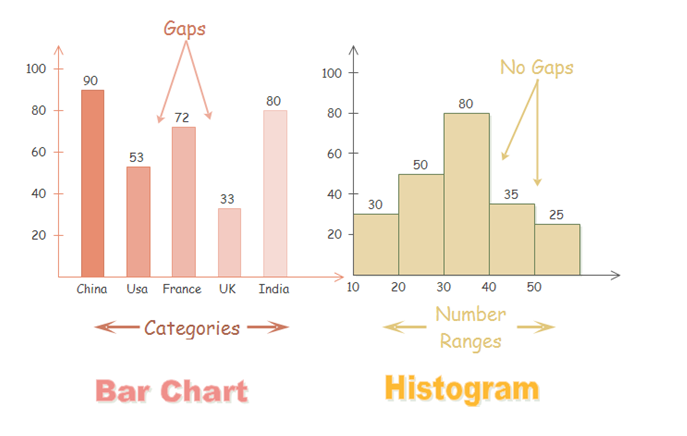
\includegraphics{4.png}
\caption{}
\end{figure}

\begin{verbatim}
Preference:https://www.edrawsoft.com/histogram-vs-bar-chart.php
\end{verbatim}

\begin{itemize}
\item
  \href{https://www.edrawsoft.com/histogram-vs-bar-chart.php}{Histograms
  VS. Bar Charts}
\item
  \href{https://www.forbes.com/sites/naomirobbins/2012/01/04/a-histogram-is-not-a-bar-chart/\#9849a526d775}{A
  Histogram is NOT a Bar Chart}
\end{itemize}

\textbf{Simple Histograms:}

\begin{itemize}
\item
  x: a numeric vector
\item
  breaks: breakpoints between histogram cells.
\end{itemize}

\begin{Shaded}
\begin{Highlighting}[]
\CommentTok{# Simple Histogram}
\KeywordTok{par}\NormalTok{(}\DataTypeTok{mfrow=}\KeywordTok{c}\NormalTok{(}\DecValTok{2}\NormalTok{,}\DecValTok{1}\NormalTok{), }\DataTypeTok{mar=}\KeywordTok{c}\NormalTok{(}\DecValTok{3}\NormalTok{,}\DecValTok{3}\NormalTok{,}\DecValTok{1}\NormalTok{,}\DecValTok{0}\NormalTok{)}\OperatorTok{+}\NormalTok{.}\DecValTok{5}\NormalTok{, }\DataTypeTok{mgp=}\KeywordTok{c}\NormalTok{(}\FloatTok{1.6}\NormalTok{,.}\DecValTok{6}\NormalTok{,}\DecValTok{0}\NormalTok{))}
\KeywordTok{hist}\NormalTok{(mtcars}\OperatorTok{$}\NormalTok{mpg,}\DataTypeTok{col=}\StringTok{"mistyrose"}\NormalTok{)}
\KeywordTok{hist}\NormalTok{(mtcars}\OperatorTok{$}\NormalTok{mpg, }\DataTypeTok{breaks =}\DecValTok{30}\NormalTok{,}\DataTypeTok{col=}\StringTok{"pink"}\NormalTok{)}
\end{Highlighting}
\end{Shaded}

\includegraphics{bookdown-demo_files/figure-latex/unnamed-chunk-51-1.pdf}

\textbf{Colored Histogram:}

\begin{Shaded}
\begin{Highlighting}[]
\KeywordTok{hist}\NormalTok{(mtcars}\OperatorTok{$}\NormalTok{mpg, }\DataTypeTok{breaks=}\DecValTok{12}\NormalTok{, }\DataTypeTok{col=}\StringTok{"mistyrose"}\NormalTok{)}
\end{Highlighting}
\end{Shaded}

\includegraphics{bookdown-demo_files/figure-latex/unnamed-chunk-52-1.pdf}

\textbf{Add a Normal Curve:}

\begin{Shaded}
\begin{Highlighting}[]
\NormalTok{x <-}\StringTok{ }\NormalTok{mtcars}\OperatorTok{$}\NormalTok{mpg }
\NormalTok{h<-}\KeywordTok{hist}\NormalTok{(x, }\DataTypeTok{breaks=}\DecValTok{10}\NormalTok{, }\DataTypeTok{col=}\StringTok{"mistyrose"}\NormalTok{, }\DataTypeTok{xlab=}\StringTok{"Miles Per Gallon"}\NormalTok{, }
   \DataTypeTok{main=}\StringTok{"Histogram with Normal Curve"}\NormalTok{) }
\NormalTok{xfit<-}\KeywordTok{seq}\NormalTok{(}\KeywordTok{min}\NormalTok{(x),}\KeywordTok{max}\NormalTok{(x),}\DataTypeTok{length=}\DecValTok{40}\NormalTok{) }
\NormalTok{yfit<-}\KeywordTok{dnorm}\NormalTok{(xfit,}\DataTypeTok{mean=}\KeywordTok{mean}\NormalTok{(x),}\DataTypeTok{sd=}\KeywordTok{sd}\NormalTok{(x)) }
\NormalTok{yfit <-}\StringTok{ }\NormalTok{yfit}\OperatorTok{*}\KeywordTok{diff}\NormalTok{(h}\OperatorTok{$}\NormalTok{mids[}\DecValTok{1}\OperatorTok{:}\DecValTok{2}\NormalTok{])}\OperatorTok{*}\KeywordTok{length}\NormalTok{(x) }
\KeywordTok{lines}\NormalTok{(xfit, yfit, }\DataTypeTok{col=}\StringTok{"red"}\NormalTok{, }\DataTypeTok{lwd=}\DecValTok{2}\NormalTok{)}
\end{Highlighting}
\end{Shaded}

\includegraphics{bookdown-demo_files/figure-latex/unnamed-chunk-53-1.pdf}

\textbf{Density plots: density():}

\begin{Shaded}
\begin{Highlighting}[]
\CommentTok{# The density data}
\NormalTok{dens <-}\StringTok{ }\KeywordTok{density}\NormalTok{(mtcars}\OperatorTok{$}\NormalTok{mpg)}
\CommentTok{# plot density}
\KeywordTok{plot}\NormalTok{(dens, }\DataTypeTok{frame =} \OtherTok{FALSE}\NormalTok{, }\DataTypeTok{col =} \StringTok{"red"}\NormalTok{, }
     \DataTypeTok{main =} \StringTok{"Density plot of mpg"}\NormalTok{) }
\end{Highlighting}
\end{Shaded}

\includegraphics{bookdown-demo_files/figure-latex/unnamed-chunk-54-1.pdf}

\textbf{Density plot using polygon():}

\begin{Shaded}
\begin{Highlighting}[]
\KeywordTok{plot}\NormalTok{(dens, }\DataTypeTok{frame =} \OtherTok{FALSE}\NormalTok{, }\DataTypeTok{col =} \StringTok{"lightblue"}\NormalTok{, }
     \DataTypeTok{main =} \StringTok{"Density plot of mpg"}\NormalTok{) }
\KeywordTok{polygon}\NormalTok{(dens, }\DataTypeTok{col =} \StringTok{"#70E500"}\NormalTok{)}
\end{Highlighting}
\end{Shaded}

\includegraphics{bookdown-demo_files/figure-latex/unnamed-chunk-55-1.pdf}

\textbf{Additional-\textgreater{}Comparing density Plots:}

Example-1:

\begin{Shaded}
\begin{Highlighting}[]
\CommentTok{#install.packages("sm")}
\KeywordTok{library}\NormalTok{(sm)}
\end{Highlighting}
\end{Shaded}

\begin{verbatim}
## Package 'sm', version 2.2-5.6: type help(sm) for summary information
\end{verbatim}

\begin{Shaded}
\begin{Highlighting}[]
\KeywordTok{sm.density.compare}\NormalTok{(iris}\OperatorTok{$}\NormalTok{Sepal.Length, iris}\OperatorTok{$}\NormalTok{Species, }\DataTypeTok{xlab=}\StringTok{"Species"}\NormalTok{)}
\KeywordTok{title}\NormalTok{(}\DataTypeTok{main=}\StringTok{"Distributions of Species"}\NormalTok{)}
\end{Highlighting}
\end{Shaded}

\includegraphics{bookdown-demo_files/figure-latex/unnamed-chunk-56-1.pdf}

Example-2:

\begin{Shaded}
\begin{Highlighting}[]
\NormalTok{x <-}\StringTok{ }\KeywordTok{seq}\NormalTok{(}\DataTypeTok{from =} \DecValTok{110}\NormalTok{, }\DataTypeTok{to =} \DecValTok{174}\NormalTok{, }\DataTypeTok{by =} \FloatTok{0.5}\NormalTok{)}
\NormalTok{y1 <-}\StringTok{ }\KeywordTok{dnorm}\NormalTok{(x, }\DataTypeTok{mean =} \DecValTok{145}\NormalTok{, }\DataTypeTok{sd =} \DecValTok{9}\NormalTok{)}
\NormalTok{y2 <-}\StringTok{ }\KeywordTok{dnorm}\NormalTok{(x, }\DataTypeTok{mean =} \DecValTok{138}\NormalTok{, }\DataTypeTok{sd =} \DecValTok{8}\NormalTok{)}
\KeywordTok{plot}\NormalTok{(x, y1, }\DataTypeTok{type=}\StringTok{"l"}\NormalTok{, }\DataTypeTok{lwd=}\DecValTok{2}\NormalTok{, }\DataTypeTok{col=}\StringTok{"mistyrose"}\NormalTok{,}
     \DataTypeTok{main=}\StringTok{"Systolic Blood Pressure Before and After Treatment"}\NormalTok{,}
     \DataTypeTok{xlab =} \StringTok{"Systolic Blood Pressure (mmHg)"}\NormalTok{,}
     \DataTypeTok{ylab =} \StringTok{"Frequency"}\NormalTok{, }\DataTypeTok{yaxt=}\StringTok{"n"}\NormalTok{,}
     \DataTypeTok{xlim =} \KeywordTok{c}\NormalTok{(}\DecValTok{110}\NormalTok{, }\DecValTok{175}\NormalTok{), }\DataTypeTok{ylim =} \KeywordTok{c}\NormalTok{(}\DecValTok{0}\NormalTok{, }\FloatTok{0.05}\NormalTok{))}
\KeywordTok{lines}\NormalTok{(x, y2)}
\KeywordTok{polygon}\NormalTok{(}\KeywordTok{c}\NormalTok{(}\DecValTok{110}\NormalTok{,x,}\DecValTok{175}\NormalTok{),}\KeywordTok{c}\NormalTok{(}\DecValTok{0}\NormalTok{,y2,}\DecValTok{0}\NormalTok{), }\DataTypeTok{col=}\StringTok{"green"}\NormalTok{,}
     \DataTypeTok{border =} \StringTok{"orange"}\NormalTok{)}
\KeywordTok{polygon}\NormalTok{(}\KeywordTok{c}\NormalTok{(}\DecValTok{117}\NormalTok{,x,}\DecValTok{175}\NormalTok{),}\KeywordTok{c}\NormalTok{(}\DecValTok{0}\NormalTok{,y1,}\DecValTok{0}\NormalTok{), }\DataTypeTok{col=}\StringTok{"lightblue"}\NormalTok{,}
     \DataTypeTok{border =} \StringTok{"orange"}\NormalTok{)}
\NormalTok{ylab=}\KeywordTok{c}\NormalTok{(}\KeywordTok{seq}\NormalTok{(}\DataTypeTok{from=}\DecValTok{0}\NormalTok{, }\DataTypeTok{to=}\DecValTok{175}\NormalTok{, }\DataTypeTok{by=}\DecValTok{25}\NormalTok{))}
\NormalTok{y=}\KeywordTok{c}\NormalTok{(}\KeywordTok{seq}\NormalTok{(}\DataTypeTok{from=}\DecValTok{0}\NormalTok{, }\DataTypeTok{to=}\FloatTok{0.05}\NormalTok{, }\DataTypeTok{length.out =} \DecValTok{8}\NormalTok{))}
\KeywordTok{axis}\NormalTok{(}\DecValTok{2}\NormalTok{,}\DataTypeTok{at=}\NormalTok{y,}\DataTypeTok{labels=}\NormalTok{ylab, }\DataTypeTok{las=}\DecValTok{1}\NormalTok{)}
\KeywordTok{text}\NormalTok{(}\DataTypeTok{x =} \DecValTok{120}\NormalTok{, }\DataTypeTok{y =} \FloatTok{0.045}\NormalTok{, }\StringTok{"- Pre-Treatment BP"}\NormalTok{, }\DataTypeTok{col =} \StringTok{"#0E51A7"}\NormalTok{, }\DataTypeTok{cex =} \FloatTok{0.9}\NormalTok{)}
\KeywordTok{text}\NormalTok{(}\DataTypeTok{x =} \DecValTok{120}\NormalTok{, }\DataTypeTok{y =} \FloatTok{0.04}\NormalTok{, }\StringTok{" - Post-Treatment BP"}\NormalTok{, }\DataTypeTok{col =} \StringTok{"firebrick3"}\NormalTok{, }\DataTypeTok{cex =} \FloatTok{0.9}\NormalTok{)}
\KeywordTok{points}\NormalTok{(}\DecValTok{109}\NormalTok{, }\FloatTok{0.0445}\NormalTok{, }\DataTypeTok{pch =} \DecValTok{15}\NormalTok{, }\DataTypeTok{col =} \StringTok{"lightblue"}\NormalTok{)}
\KeywordTok{points}\NormalTok{(}\DecValTok{109}\NormalTok{, }\FloatTok{0.0395}\NormalTok{, }\DataTypeTok{pch =} \DecValTok{15}\NormalTok{, }\DataTypeTok{col =} \StringTok{"lightblue"}\NormalTok{)}
\end{Highlighting}
\end{Shaded}

\includegraphics{bookdown-demo_files/figure-latex/unnamed-chunk-57-1.pdf}

\chapter{Default Line Plots in R}\label{default-line-plots-in-r}

Note that the function \texttt{lines()} need a \texttt{plot()}.

\textbf{Basic line plots:}

Example-1:

\begin{Shaded}
\begin{Highlighting}[]
\KeywordTok{par}\NormalTok{(}\DataTypeTok{mfrow=}\KeywordTok{c}\NormalTok{(}\DecValTok{2}\NormalTok{,}\DecValTok{1}\NormalTok{), }\DataTypeTok{mar=}\KeywordTok{c}\NormalTok{(}\DecValTok{3}\NormalTok{,}\DecValTok{3}\NormalTok{,}\DecValTok{1}\NormalTok{,}\DecValTok{0}\NormalTok{)}\OperatorTok{+}\NormalTok{.}\DecValTok{5}\NormalTok{, }\DataTypeTok{mgp=}\KeywordTok{c}\NormalTok{(}\FloatTok{1.6}\NormalTok{,.}\DecValTok{6}\NormalTok{,}\DecValTok{0}\NormalTok{))}
\NormalTok{x <-}\StringTok{ }\DecValTok{1}\OperatorTok{:}\DecValTok{10}
\NormalTok{y1 <-}\StringTok{ }\NormalTok{x}\OperatorTok{*}\NormalTok{x}
\NormalTok{y2  <-}\StringTok{ }\DecValTok{3}\OperatorTok{*}\NormalTok{y1}
\CommentTok{# Basic stair steps plot }
\KeywordTok{plot}\NormalTok{(x, y1, }\DataTypeTok{type =} \StringTok{"S"}\NormalTok{,}\DataTypeTok{plot=}\StringTok{"pink"}\NormalTok{)}
\end{Highlighting}
\end{Shaded}

\begin{verbatim}
## Warning in plot.window(...): "plot" is not a graphical parameter
\end{verbatim}

\begin{verbatim}
## Warning in plot.xy(xy, type, ...): "plot" is not a graphical parameter
\end{verbatim}

\begin{verbatim}
## Warning in axis(side = side, at = at, labels = labels, ...): "plot" is not
## a graphical parameter

## Warning in axis(side = side, at = at, labels = labels, ...): "plot" is not
## a graphical parameter
\end{verbatim}

\begin{verbatim}
## Warning in box(...): "plot" is not a graphical parameter
\end{verbatim}

\begin{verbatim}
## Warning in title(...): "plot" is not a graphical parameter
\end{verbatim}

\begin{Shaded}
\begin{Highlighting}[]
\CommentTok{# Points and line}
\KeywordTok{plot}\NormalTok{(x, y1, }\DataTypeTok{type =} \StringTok{"b"}\NormalTok{, }\DataTypeTok{pch =} \DecValTok{19}\NormalTok{, }
     \DataTypeTok{col =} \StringTok{"blue"}\NormalTok{, }\DataTypeTok{xlab =} \StringTok{"x"}\NormalTok{, }\DataTypeTok{ylab =} \StringTok{"y"}\NormalTok{)}
\end{Highlighting}
\end{Shaded}

\includegraphics{bookdown-demo_files/figure-latex/unnamed-chunk-58-1.pdf}

Example-2: As functions for different types

\begin{Shaded}
\begin{Highlighting}[]
\NormalTok{x <-}\StringTok{ }\KeywordTok{c}\NormalTok{(}\DecValTok{1}\OperatorTok{:}\DecValTok{5}\NormalTok{); y <-}\StringTok{ }\NormalTok{x}\OperatorTok{*}\NormalTok{x }\CommentTok{# create example data }
\KeywordTok{par}\NormalTok{(}\DataTypeTok{pch=}\DecValTok{22}\NormalTok{, }\DataTypeTok{col=}\StringTok{"blue"}\NormalTok{) }\CommentTok{# plotting symbol and color }
\KeywordTok{par}\NormalTok{(}\DataTypeTok{mfrow=}\KeywordTok{c}\NormalTok{(}\DecValTok{2}\NormalTok{,}\DecValTok{4}\NormalTok{)) }\CommentTok{# all plots on one page }
\NormalTok{opts =}\StringTok{ }\KeywordTok{c}\NormalTok{(}\StringTok{"p"}\NormalTok{,}\StringTok{"l"}\NormalTok{,}\StringTok{"o"}\NormalTok{,}\StringTok{"b"}\NormalTok{,}\StringTok{"c"}\NormalTok{,}\StringTok{"s"}\NormalTok{,}\StringTok{"S"}\NormalTok{,}\StringTok{"h"}\NormalTok{) }
\ControlFlowTok{for}\NormalTok{(i }\ControlFlowTok{in} \DecValTok{1}\OperatorTok{:}\KeywordTok{length}\NormalTok{(opts))\{ }
\NormalTok{  heading =}\StringTok{ }\KeywordTok{paste}\NormalTok{(}\StringTok{"type="}\NormalTok{,opts[i]) }
  \KeywordTok{plot}\NormalTok{(x, y, }\DataTypeTok{type=}\StringTok{"n"}\NormalTok{, }\DataTypeTok{main=}\NormalTok{heading) }
  \KeywordTok{lines}\NormalTok{(x, y, }\DataTypeTok{type=}\NormalTok{opts[i]) }
\NormalTok{\}}
\end{Highlighting}
\end{Shaded}

\includegraphics{bookdown-demo_files/figure-latex/unnamed-chunk-59-1.pdf}

Example-3: Plot the points type=``''

\begin{Shaded}
\begin{Highlighting}[]
\NormalTok{x <-}\StringTok{ }\KeywordTok{c}\NormalTok{(}\DecValTok{1}\OperatorTok{:}\DecValTok{5}\NormalTok{); y <-}\StringTok{ }\NormalTok{x}\OperatorTok{*}\NormalTok{x }\CommentTok{# create example data}
\KeywordTok{par}\NormalTok{(}\DataTypeTok{pch=}\DecValTok{22}\NormalTok{, }\DataTypeTok{col=}\StringTok{"#00AE68"}\NormalTok{) }\CommentTok{# plotting symbol and color }
\KeywordTok{par}\NormalTok{(}\DataTypeTok{mfrow=}\KeywordTok{c}\NormalTok{(}\DecValTok{2}\NormalTok{,}\DecValTok{4}\NormalTok{)) }\CommentTok{# all plots on one page }
\NormalTok{opts =}\StringTok{ }\KeywordTok{c}\NormalTok{(}\StringTok{"p"}\NormalTok{,}\StringTok{"l"}\NormalTok{,}\StringTok{"o"}\NormalTok{,}\StringTok{"b"}\NormalTok{,}\StringTok{"c"}\NormalTok{,}\StringTok{"s"}\NormalTok{,}\StringTok{"S"}\NormalTok{,}\StringTok{"h"}\NormalTok{) }

\ControlFlowTok{for}\NormalTok{(i }\ControlFlowTok{in} \DecValTok{1}\OperatorTok{:}\KeywordTok{length}\NormalTok{(opts))\{ }
\NormalTok{  heading =}\StringTok{ }\KeywordTok{paste}\NormalTok{(}\StringTok{"type="}\NormalTok{,opts[i]) }
  \KeywordTok{plot}\NormalTok{(x, y, }\DataTypeTok{main=}\NormalTok{heading) }
  \KeywordTok{lines}\NormalTok{(x, y, }\DataTypeTok{type=}\NormalTok{opts[i]) \}}
\end{Highlighting}
\end{Shaded}

\includegraphics{bookdown-demo_files/figure-latex/unnamed-chunk-60-1.pdf}

\textbf{Multiple lines plots:}

Example-1:

\begin{Shaded}
\begin{Highlighting}[]
\CommentTok{# First line}
\NormalTok{x <-}\StringTok{ }\DecValTok{1}\OperatorTok{:}\DecValTok{10}
\NormalTok{y1 <-}\StringTok{ }\NormalTok{(x}\OperatorTok{*}\NormalTok{x)}
\KeywordTok{plot}\NormalTok{(x, y1, }\DataTypeTok{type =} \StringTok{"b"}\NormalTok{, }\DataTypeTok{frame =} \OtherTok{FALSE}\NormalTok{, }\DataTypeTok{pch =} \DecValTok{19}\NormalTok{, }
     \DataTypeTok{col =} \StringTok{"red"}\NormalTok{, }\DataTypeTok{xlab =} \StringTok{"x"}\NormalTok{, }\DataTypeTok{ylab =} \StringTok{"y"}\NormalTok{)}
\CommentTok{# A second line}
\KeywordTok{lines}\NormalTok{(x, y2, }\DataTypeTok{pch =} \DecValTok{18}\NormalTok{, }\DataTypeTok{col =} \StringTok{"blue"}\NormalTok{, }\DataTypeTok{type =} \StringTok{"b"}\NormalTok{, }\DataTypeTok{lty =} \DecValTok{2}\NormalTok{)}
\CommentTok{# Add a legend to the plot}
\KeywordTok{legend}\NormalTok{(}\StringTok{"topleft"}\NormalTok{, }\DataTypeTok{legend=}\KeywordTok{c}\NormalTok{(}\StringTok{"Line 1"}\NormalTok{, }\StringTok{"Line 2"}\NormalTok{),}
       \DataTypeTok{col=}\KeywordTok{c}\NormalTok{(}\StringTok{"red"}\NormalTok{, }\StringTok{"blue"}\NormalTok{), }\DataTypeTok{lty =} \DecValTok{1}\OperatorTok{:}\DecValTok{2}\NormalTok{, }\DataTypeTok{cex=}\FloatTok{0.8}\NormalTok{)}
\end{Highlighting}
\end{Shaded}

\includegraphics{bookdown-demo_files/figure-latex/unnamed-chunk-61-1.pdf}

Example-2: As functions for different types

\begin{Shaded}
\begin{Highlighting}[]
\CommentTok{# Create Line Chart}
\CommentTok{# convert factor to numeric for convenience }
\NormalTok{Orange}\OperatorTok{$}\NormalTok{Tree <-}\StringTok{ }\KeywordTok{as.numeric}\NormalTok{(Orange}\OperatorTok{$}\NormalTok{Tree) }
\NormalTok{ntrees <-}\StringTok{ }\KeywordTok{max}\NormalTok{(Orange}\OperatorTok{$}\NormalTok{Tree)}

\CommentTok{# get the range for the x and y axis }
\NormalTok{xrange <-}\StringTok{ }\KeywordTok{range}\NormalTok{(Orange}\OperatorTok{$}\NormalTok{age) }
\NormalTok{yrange <-}\StringTok{ }\KeywordTok{range}\NormalTok{(Orange}\OperatorTok{$}\NormalTok{circumference) }

\CommentTok{# set up the plot }
\KeywordTok{plot}\NormalTok{(xrange, yrange, }\DataTypeTok{type=}\StringTok{"n"}\NormalTok{, }\DataTypeTok{xlab=}\StringTok{"Age (days)"}\NormalTok{,}
   \DataTypeTok{ylab=}\StringTok{"Circumference (mm)"}\NormalTok{ ) }
\NormalTok{colors <-}\StringTok{ }\KeywordTok{rainbow}\NormalTok{(ntrees) }
\NormalTok{linetype <-}\StringTok{ }\KeywordTok{c}\NormalTok{(}\DecValTok{1}\OperatorTok{:}\NormalTok{ntrees) }
\NormalTok{plotchar <-}\StringTok{ }\KeywordTok{seq}\NormalTok{(}\DecValTok{18}\NormalTok{,}\DecValTok{18}\OperatorTok{+}\NormalTok{ntrees,}\DecValTok{1}\NormalTok{)}

\CommentTok{# add lines }
\ControlFlowTok{for}\NormalTok{ (i }\ControlFlowTok{in} \DecValTok{1}\OperatorTok{:}\NormalTok{ntrees) \{ }
\NormalTok{  tree <-}\StringTok{ }\KeywordTok{subset}\NormalTok{(Orange, Tree}\OperatorTok{==}\NormalTok{i) }
  \KeywordTok{lines}\NormalTok{(tree}\OperatorTok{$}\NormalTok{age, tree}\OperatorTok{$}\NormalTok{circumference, }\DataTypeTok{type=}\StringTok{"b"}\NormalTok{, }\DataTypeTok{lwd=}\FloatTok{1.5}\NormalTok{,}
    \DataTypeTok{lty=}\NormalTok{linetype[i], }\DataTypeTok{col=}\NormalTok{colors[i], }\DataTypeTok{pch=}\NormalTok{plotchar[i]) }
\NormalTok{\} }

\CommentTok{# add a title and subtitle }
\KeywordTok{title}\NormalTok{(}\StringTok{"Tree Growth"}\NormalTok{, }\StringTok{"example of line plot"}\NormalTok{)}

\CommentTok{# add a legend }
\KeywordTok{legend}\NormalTok{(xrange[}\DecValTok{1}\NormalTok{], yrange[}\DecValTok{2}\NormalTok{], }\DecValTok{1}\OperatorTok{:}\NormalTok{ntrees, }\DataTypeTok{cex=}\FloatTok{0.8}\NormalTok{, }\DataTypeTok{col=}\NormalTok{colors,}
   \DataTypeTok{pch=}\NormalTok{plotchar, }\DataTypeTok{lty=}\NormalTok{linetype, }\DataTypeTok{title=}\StringTok{"Tree"}\NormalTok{)}
\end{Highlighting}
\end{Shaded}

\includegraphics{bookdown-demo_files/figure-latex/unnamed-chunk-62-1.pdf}

\chapter{Default Scatter Plots in R}\label{default-scatter-plots-in-r}

\textbf{R base scatter plot: plot():}

Example-1:

\begin{Shaded}
\begin{Highlighting}[]
\KeywordTok{par}\NormalTok{(}\DataTypeTok{mfrow=}\KeywordTok{c}\NormalTok{(}\DecValTok{2}\NormalTok{,}\DecValTok{1}\NormalTok{), }\DataTypeTok{mar=}\KeywordTok{c}\NormalTok{(}\DecValTok{3}\NormalTok{,}\DecValTok{3}\NormalTok{,}\DecValTok{1}\NormalTok{,}\DecValTok{0}\NormalTok{)}\OperatorTok{+}\NormalTok{.}\DecValTok{5}\NormalTok{, }\DataTypeTok{mgp=}\KeywordTok{c}\NormalTok{(}\FloatTok{1.6}\NormalTok{,.}\DecValTok{6}\NormalTok{,}\DecValTok{0}\NormalTok{))}
\NormalTok{x <-}\StringTok{ }\NormalTok{mtcars}\OperatorTok{$}\NormalTok{hp}
\NormalTok{y <-}\StringTok{ }\NormalTok{mtcars}\OperatorTok{$}\NormalTok{mpg}
\CommentTok{# Plot with main and axis titles}
\CommentTok{# Change point shape (pch = 19) and remove frame.}
\KeywordTok{plot}\NormalTok{(x, y, }\DataTypeTok{main =} \StringTok{"Main title"}\NormalTok{,}
     \DataTypeTok{xlab =} \StringTok{"X axis title"}\NormalTok{, }\DataTypeTok{ylab =} \StringTok{"Y axis title"}\NormalTok{,}
     \DataTypeTok{pch =} \DecValTok{19}\NormalTok{, }\DataTypeTok{frame =} \OtherTok{FALSE}\NormalTok{,}\DataTypeTok{col=}\StringTok{"#FFC000"}\NormalTok{)}
\CommentTok{# Add regression line}
\KeywordTok{plot}\NormalTok{(x, y, }\DataTypeTok{main =} \StringTok{"Main title"}\NormalTok{,}
     \DataTypeTok{xlab =} \StringTok{"X axis title"}\NormalTok{, }\DataTypeTok{ylab =} \StringTok{"Y axis title"}\NormalTok{,}
     \DataTypeTok{pch =} \DecValTok{19}\NormalTok{, }\DataTypeTok{frame =} \OtherTok{FALSE}\NormalTok{,}\DataTypeTok{col=}\StringTok{"#7573D9"}\NormalTok{)}
\KeywordTok{abline}\NormalTok{(}\KeywordTok{lm}\NormalTok{(y }\OperatorTok{~}\StringTok{ }\NormalTok{x, }\DataTypeTok{data =}\NormalTok{ mtcars), }\DataTypeTok{col =} \StringTok{"blue"}\NormalTok{)}
\end{Highlighting}
\end{Shaded}

\includegraphics{bookdown-demo_files/figure-latex/unnamed-chunk-63-1.pdf}

Example-2:

\begin{Shaded}
\begin{Highlighting}[]
\NormalTok{x <-}\StringTok{ }\NormalTok{mtcars}\OperatorTok{$}\NormalTok{hp}
\NormalTok{y <-}\StringTok{ }\NormalTok{mtcars}\OperatorTok{$}\NormalTok{mpg}
\CommentTok{# Add loess fit}
\KeywordTok{plot}\NormalTok{(x, y, }\DataTypeTok{main =} \StringTok{"Main title"}\NormalTok{,}
     \DataTypeTok{xlab =} \StringTok{"X axis title"}\NormalTok{, }\DataTypeTok{ylab =} \StringTok{"Y axis title"}\NormalTok{,}
     \DataTypeTok{pch =} \DecValTok{19}\NormalTok{, }\DataTypeTok{frame =} \OtherTok{FALSE}\NormalTok{,}\DataTypeTok{col=}\StringTok{"red"}\NormalTok{)}
\KeywordTok{lines}\NormalTok{(}\KeywordTok{lowess}\NormalTok{(x, y), }\DataTypeTok{col =} \StringTok{"blue"}\NormalTok{)}
\end{Highlighting}
\end{Shaded}

\includegraphics{bookdown-demo_files/figure-latex/unnamed-chunk-64-1.pdf}

\textbf{Addtional-\textgreater{}Enhanced scatter plots:}

The components of the plot contains:

\begin{itemize}
\tightlist
\item
  the points
\item
  the regression line (in green)
\item
  the smoothed conditional spread (in red dashed line)
\item
  the non-parametric regression smooth (solid line, red)
\end{itemize}

\begin{Shaded}
\begin{Highlighting}[]
\CommentTok{#install.packages("car")}
\KeywordTok{library}\NormalTok{(}\StringTok{"car"}\NormalTok{)}
\end{Highlighting}
\end{Shaded}

\begin{verbatim}
## Loading required package: carData
\end{verbatim}

\begin{Shaded}
\begin{Highlighting}[]
\KeywordTok{scatterplot}\NormalTok{(wt }\OperatorTok{~}\StringTok{ }\NormalTok{mpg, }\DataTypeTok{data =}\NormalTok{ mtcars)}
\end{Highlighting}
\end{Shaded}

\includegraphics{bookdown-demo_files/figure-latex/unnamed-chunk-65-1.pdf}

\chapter{Default Scatter Plot Matrices in
R}\label{default-scatter-plot-matrices-in-r}

\textbf{Scatter Plot Matrices:}

\begin{Shaded}
\begin{Highlighting}[]
\KeywordTok{par}\NormalTok{(}\DataTypeTok{mfrow=}\KeywordTok{c}\NormalTok{(}\DecValTok{2}\NormalTok{,}\DecValTok{1}\NormalTok{))}
\KeywordTok{pairs}\NormalTok{(}\OperatorTok{~}\NormalTok{mpg}\OperatorTok{+}\NormalTok{disp}\OperatorTok{+}\NormalTok{drat}\OperatorTok{+}\NormalTok{wt,}\DataTypeTok{data=}\NormalTok{mtcars, }
   \DataTypeTok{main=}\StringTok{"Simple Scatterplot Matrix"}\NormalTok{)}
\end{Highlighting}
\end{Shaded}

\includegraphics{bookdown-demo_files/figure-latex/unnamed-chunk-66-1.pdf}

\begin{Shaded}
\begin{Highlighting}[]
\KeywordTok{pairs}\NormalTok{(}\OperatorTok{~}\NormalTok{mpg}\OperatorTok{+}\NormalTok{disp}\OperatorTok{+}\NormalTok{drat}\OperatorTok{+}\NormalTok{wt,}\DataTypeTok{data=}\NormalTok{mtcars,}\DataTypeTok{lower.panel =} \OtherTok{NULL}\NormalTok{,}
   \DataTypeTok{main=}\StringTok{"Simple Scatterplot Matrix"}\NormalTok{)}
\end{Highlighting}
\end{Shaded}

\includegraphics{bookdown-demo_files/figure-latex/unnamed-chunk-66-2.pdf}

\textbf{Color points by groups Scatter plots:}

\begin{Shaded}
\begin{Highlighting}[]
\NormalTok{my_col <-}\StringTok{ }\KeywordTok{c}\NormalTok{(}\StringTok{"#00AFBB"}\NormalTok{, }\StringTok{"#E7B800"}\NormalTok{, }\StringTok{"#FC4E07"}\NormalTok{)  }
\KeywordTok{pairs}\NormalTok{(iris[,}\DecValTok{1}\OperatorTok{:}\DecValTok{4}\NormalTok{], }\DataTypeTok{pch =} \DecValTok{19}\NormalTok{,  }\DataTypeTok{cex =} \FloatTok{0.5}\NormalTok{,}
      \DataTypeTok{col =}\NormalTok{ my_col[iris}\OperatorTok{$}\NormalTok{Species],}
      \DataTypeTok{lower.panel=}\OtherTok{NULL}\NormalTok{)}
\end{Highlighting}
\end{Shaded}

\includegraphics{bookdown-demo_files/figure-latex/unnamed-chunk-67-1.pdf}

\textbf{Add correlations on the lower panels: }

\begin{Shaded}
\begin{Highlighting}[]
\CommentTok{# Correlation panel}
\NormalTok{my_col <-}\StringTok{ }\KeywordTok{c}\NormalTok{(}\StringTok{"#00AFBB"}\NormalTok{, }\StringTok{"#E7B800"}\NormalTok{, }\StringTok{"#FC4E07"}\NormalTok{) }
\NormalTok{panel.cor <-}\StringTok{ }\ControlFlowTok{function}\NormalTok{(x, y)\{}
\NormalTok{    usr <-}\StringTok{ }\KeywordTok{par}\NormalTok{(}\StringTok{"usr"}\NormalTok{); }\KeywordTok{on.exit}\NormalTok{(}\KeywordTok{par}\NormalTok{(usr))}
    \KeywordTok{par}\NormalTok{(}\DataTypeTok{usr =} \KeywordTok{c}\NormalTok{(}\DecValTok{0}\NormalTok{, }\DecValTok{1}\NormalTok{, }\DecValTok{0}\NormalTok{, }\DecValTok{1}\NormalTok{))}
\NormalTok{    r <-}\StringTok{ }\KeywordTok{round}\NormalTok{(}\KeywordTok{cor}\NormalTok{(x, y), }\DataTypeTok{digits=}\DecValTok{2}\NormalTok{)}
\NormalTok{    txt <-}\StringTok{ }\KeywordTok{paste0}\NormalTok{(}\StringTok{"R = "}\NormalTok{, r)}
\NormalTok{    cex.cor <-}\StringTok{ }\FloatTok{0.8}\OperatorTok{/}\KeywordTok{strwidth}\NormalTok{(txt)}
    \KeywordTok{text}\NormalTok{(}\FloatTok{0.5}\NormalTok{, }\FloatTok{0.5}\NormalTok{, txt, }\DataTypeTok{cex =}\NormalTok{ cex.cor }\OperatorTok{*}\StringTok{ }\NormalTok{r)}
\NormalTok{\}}
\CommentTok{# Customize upper panel}
\NormalTok{upper.panel<-}\ControlFlowTok{function}\NormalTok{(x, y)\{}
  \KeywordTok{points}\NormalTok{(x,y, }\DataTypeTok{pch =} \DecValTok{19}\NormalTok{, }\DataTypeTok{col =}\NormalTok{ my_col[iris}\OperatorTok{$}\NormalTok{Species])}
\NormalTok{\}}
\CommentTok{# Create the plots}
\KeywordTok{pairs}\NormalTok{(iris[,}\DecValTok{1}\OperatorTok{:}\DecValTok{4}\NormalTok{], }
      \DataTypeTok{lower.panel =}\NormalTok{ panel.cor,}
      \DataTypeTok{upper.panel =}\NormalTok{ upper.panel)}
\end{Highlighting}
\end{Shaded}

\includegraphics{bookdown-demo_files/figure-latex/unnamed-chunk-68-1.pdf}

\textbf{Add correlations on the scatter plots:}

\begin{Shaded}
\begin{Highlighting}[]
\NormalTok{my_col <-}\StringTok{ }\KeywordTok{c}\NormalTok{(}\StringTok{"#00AFBB"}\NormalTok{, }\StringTok{"#E7B800"}\NormalTok{, }\StringTok{"#FC4E07"}\NormalTok{)}
\CommentTok{# Customize upper panel}
\NormalTok{upper.panel<-}\ControlFlowTok{function}\NormalTok{(x, y)\{}
  \KeywordTok{points}\NormalTok{(x,y, }\DataTypeTok{pch=}\DecValTok{19}\NormalTok{, }\DataTypeTok{col=}\KeywordTok{c}\NormalTok{(}\StringTok{"red"}\NormalTok{, }\StringTok{"green3"}\NormalTok{, }\StringTok{"blue"}\NormalTok{)[iris}\OperatorTok{$}\NormalTok{Species])}
\NormalTok{  r <-}\StringTok{ }\KeywordTok{round}\NormalTok{(}\KeywordTok{cor}\NormalTok{(x, y), }\DataTypeTok{digits=}\DecValTok{2}\NormalTok{)}
\NormalTok{  txt <-}\StringTok{ }\KeywordTok{paste0}\NormalTok{(}\StringTok{"R = "}\NormalTok{, r)}
\NormalTok{  usr <-}\StringTok{ }\KeywordTok{par}\NormalTok{(}\StringTok{"usr"}\NormalTok{); }\KeywordTok{on.exit}\NormalTok{(}\KeywordTok{par}\NormalTok{(usr))}
  \KeywordTok{par}\NormalTok{(}\DataTypeTok{usr =} \KeywordTok{c}\NormalTok{(}\DecValTok{0}\NormalTok{, }\DecValTok{1}\NormalTok{, }\DecValTok{0}\NormalTok{, }\DecValTok{1}\NormalTok{))}
  \KeywordTok{text}\NormalTok{(}\FloatTok{0.5}\NormalTok{, }\FloatTok{0.9}\NormalTok{, txt)}
\NormalTok{\}}
\KeywordTok{pairs}\NormalTok{(iris[,}\DecValTok{1}\OperatorTok{:}\DecValTok{4}\NormalTok{], }\DataTypeTok{lower.panel =} \OtherTok{NULL}\NormalTok{, }
      \DataTypeTok{upper.panel =}\NormalTok{ upper.panel)}
\end{Highlighting}
\end{Shaded}

\includegraphics{bookdown-demo_files/figure-latex/unnamed-chunk-69-1.pdf}

\textbf{Additional-\textgreater{} the R package psych:}

\begin{Shaded}
\begin{Highlighting}[]
\CommentTok{#install.packages("psych")}
\KeywordTok{library}\NormalTok{(psych)}
\end{Highlighting}
\end{Shaded}

\begin{verbatim}
## 
## Attaching package: 'psych'
\end{verbatim}

\begin{verbatim}
## The following object is masked from 'package:car':
## 
##     logit
\end{verbatim}

\begin{Shaded}
\begin{Highlighting}[]
\KeywordTok{pairs.panels}\NormalTok{(iris[,}\OperatorTok{-}\DecValTok{5}\NormalTok{], }
             \DataTypeTok{method =} \StringTok{"pearson"}\NormalTok{, }\CommentTok{# correlation method}
             \DataTypeTok{hist.col =} \StringTok{"#52E932"}\NormalTok{,}
             \DataTypeTok{density =} \OtherTok{TRUE}\NormalTok{,  }\CommentTok{# show density plots}
             \DataTypeTok{ellipses =} \OtherTok{TRUE} \CommentTok{# show correlation ellipses}
\NormalTok{             )}
\end{Highlighting}
\end{Shaded}

\includegraphics{bookdown-demo_files/figure-latex/unnamed-chunk-70-1.pdf}

\chapter{Strip charts:1-D scatter
plots}\label{strip-charts1-d-scatter-plots}

Formula:

\begin{quote}
stripchart(x, data = NULL method = ``overplot'', jitter = 0.1)
\end{quote}

\begin{itemize}
\tightlist
\item
  x: the data from which the plots are to be produced. Allowed values
  are one or a list of numeric vector, each corresponding to a component
  plot.
\item
  data: a data.frame (or list) from which the variables in x should be
  taken.
\item
  Method: the method to be used to separate coincident points. Allowed
  values are one of ``overplot'', ``jitter'' or ``stack''.
\item
  jitter: when method = ``jitter'' is used, jitter gives the amount of
  jittering applied.
\end{itemize}

Example-1:

\begin{Shaded}
\begin{Highlighting}[]
\CommentTok{# Plot len by dose}
\KeywordTok{stripchart}\NormalTok{(len }\OperatorTok{~}\StringTok{ }\NormalTok{dose, }\DataTypeTok{data =}\NormalTok{ ToothGrowth,}
         \DataTypeTok{pch =} \DecValTok{19}\NormalTok{, }\DataTypeTok{frame =} \OtherTok{FALSE}\NormalTok{,}\DataTypeTok{col=}\StringTok{"orange"}\NormalTok{)}
\end{Highlighting}
\end{Shaded}

\includegraphics{bookdown-demo_files/figure-latex/unnamed-chunk-71-1.pdf}

Example-2:

\begin{Shaded}
\begin{Highlighting}[]
\CommentTok{# Vertical plot using method = "jitter"}
\KeywordTok{stripchart}\NormalTok{(len }\OperatorTok{~}\StringTok{ }\NormalTok{dose, }\DataTypeTok{data =}\NormalTok{ ToothGrowth,}
         \DataTypeTok{pch =} \DecValTok{19}\NormalTok{, }\DataTypeTok{frame =} \OtherTok{FALSE}\NormalTok{, }\DataTypeTok{vertical =} \OtherTok{TRUE}\NormalTok{,}
         \DataTypeTok{method =} \StringTok{"jitter"}\NormalTok{,}\DataTypeTok{col=}\StringTok{"blue"}\NormalTok{)}
\end{Highlighting}
\end{Shaded}

\includegraphics{bookdown-demo_files/figure-latex/unnamed-chunk-72-1.pdf}

Example-3:

\begin{Shaded}
\begin{Highlighting}[]
\CommentTok{# Change point shapes (pch) and colors by groups}
\CommentTok{# add main title and axis labels}
\KeywordTok{stripchart}\NormalTok{(len }\OperatorTok{~}\StringTok{ }\NormalTok{dose, }\DataTypeTok{data =}\NormalTok{ ToothGrowth,}
         \DataTypeTok{frame =} \OtherTok{FALSE}\NormalTok{, }\DataTypeTok{vertical =} \OtherTok{TRUE}\NormalTok{,}
         \DataTypeTok{method =} \StringTok{"jitter"}\NormalTok{, }\DataTypeTok{pch =} \KeywordTok{c}\NormalTok{(}\DecValTok{21}\NormalTok{, }\DecValTok{18}\NormalTok{, }\DecValTok{16}\NormalTok{),}
         \DataTypeTok{col =} \KeywordTok{c}\NormalTok{(}\StringTok{"#00BF32"}\NormalTok{, }\StringTok{"#E69F00"}\NormalTok{, }\StringTok{"#56B4E9"}\NormalTok{),}
         \DataTypeTok{main =} \StringTok{"Length by dose"}\NormalTok{, }\DataTypeTok{xlab =} \StringTok{"Dose"}\NormalTok{, }\DataTypeTok{ylab =} \StringTok{"Length"}\NormalTok{)}
\end{Highlighting}
\end{Shaded}

\includegraphics{bookdown-demo_files/figure-latex/unnamed-chunk-73-1.pdf}

\chapter{Default Dot Plots in R}\label{default-dot-plots-in-r}

Formula:

\begin{quote}
dotchart(x, labels = NULL, groups = NULL, gcolor = par(``fg''), color =
par(``fg''))
\end{quote}

\textbf{Simple Dot Plots numeric vectors: }

Example-1:

\begin{Shaded}
\begin{Highlighting}[]
\CommentTok{# Simple Dot Plot}
\KeywordTok{dotchart}\NormalTok{(mtcars}\OperatorTok{$}\NormalTok{mpg,}\DataTypeTok{labels=}\KeywordTok{row.names}\NormalTok{(mtcars),}\DataTypeTok{cex=}\NormalTok{.}\DecValTok{7}\NormalTok{,}
   \DataTypeTok{main=}\StringTok{"Gas Milage for Car Models"}\NormalTok{, }
   \DataTypeTok{xlab=}\StringTok{"Miles Per Gallon"}\NormalTok{)}
\end{Highlighting}
\end{Shaded}

\includegraphics{bookdown-demo_files/figure-latex/unnamed-chunk-74-1.pdf}

Example-2:

\begin{Shaded}
\begin{Highlighting}[]
\CommentTok{# Plot and color by groups cyl}
\NormalTok{grps <-}\StringTok{ }\KeywordTok{as.factor}\NormalTok{(mtcars}\OperatorTok{$}\NormalTok{cyl)}
\NormalTok{my_cols <-}\StringTok{ }\KeywordTok{c}\NormalTok{(}\StringTok{"#0776A0"}\NormalTok{, }\StringTok{"#FFA100"}\NormalTok{, }\StringTok{"#6E0069"}\NormalTok{)}
\KeywordTok{dotchart}\NormalTok{(mtcars}\OperatorTok{$}\NormalTok{mpg, }\DataTypeTok{labels =} \KeywordTok{row.names}\NormalTok{(mtcars),}
         \DataTypeTok{groups =}\NormalTok{ grps, }\DataTypeTok{gcolor =}\NormalTok{ my_cols,}
         \DataTypeTok{color =}\NormalTok{ my_cols[grps],}
         \DataTypeTok{cex =} \FloatTok{0.6}\NormalTok{,  }\DataTypeTok{pch =} \DecValTok{19}\NormalTok{, }\DataTypeTok{xlab =} \StringTok{"mpg"}\NormalTok{)}
\end{Highlighting}
\end{Shaded}

\includegraphics{bookdown-demo_files/figure-latex/unnamed-chunk-75-1.pdf}

\textbf{Dot Plot matrix: }

\begin{Shaded}
\begin{Highlighting}[]
\KeywordTok{dotchart}\NormalTok{(VADeaths, }\DataTypeTok{cex =} \FloatTok{0.6}\NormalTok{,}
         \DataTypeTok{main =} \StringTok{"Death Rates in Virginia - 1940"}\NormalTok{)}
\end{Highlighting}
\end{Shaded}

\includegraphics{bookdown-demo_files/figure-latex/unnamed-chunk-76-1.pdf}

\chapter{Default Pie Charts in R}\label{default-pie-charts-in-r}

Formula:

\begin{quote}
pie(x, labels = names(x), radius = 0.8)
\end{quote}

\begin{itemize}
\tightlist
\item
  x: a vector of non-negative numerical quantities. The values in x are
  displayed as the areas of pie slices.
\item
  labels: character strings giving names for the slices.
\item
  radius: radius of the pie circle. If the character strings labeling
  the slices are long it may be necessary to use a smaller radius.
\end{itemize}

\textbf{Basic pie charts: -\textgreater{} pie()}

Example-1:

\begin{Shaded}
\begin{Highlighting}[]
\NormalTok{df <-}\StringTok{ }\KeywordTok{data.frame}\NormalTok{(}
  \DataTypeTok{group =} \KeywordTok{c}\NormalTok{(}\StringTok{"Male"}\NormalTok{, }\StringTok{"Female"}\NormalTok{, }\StringTok{"Child"}\NormalTok{),}
  \DataTypeTok{value =} \KeywordTok{c}\NormalTok{(}\DecValTok{35}\NormalTok{, }\DecValTok{45}\NormalTok{, }\DecValTok{20}\NormalTok{)}
\NormalTok{  )}
\NormalTok{df}
\end{Highlighting}
\end{Shaded}

\begin{verbatim}
##    group value
## 1   Male    35
## 2 Female    45
## 3  Child    20
\end{verbatim}

\begin{Shaded}
\begin{Highlighting}[]
\KeywordTok{pie}\NormalTok{(df}\OperatorTok{$}\NormalTok{value, }\DataTypeTok{labels =}\NormalTok{ df}\OperatorTok{$}\NormalTok{group, }\DataTypeTok{radius =} \DecValTok{1}\NormalTok{,}\DataTypeTok{col=}\KeywordTok{c}\NormalTok{(}\StringTok{"#AA6F39"}\NormalTok{,}\StringTok{"#2F4073"}\NormalTok{,}\StringTok{"#2B823A"}\NormalTok{))}
\end{Highlighting}
\end{Shaded}

\includegraphics{bookdown-demo_files/figure-latex/unnamed-chunk-77-1.pdf}

Example-2:

\begin{Shaded}
\begin{Highlighting}[]
\CommentTok{# Change colors}
\KeywordTok{pie}\NormalTok{(df}\OperatorTok{$}\NormalTok{value, }\DataTypeTok{labels =}\NormalTok{ df}\OperatorTok{$}\NormalTok{group, }\DataTypeTok{radius =} \DecValTok{1}\NormalTok{,}
    \DataTypeTok{col =} \KeywordTok{c}\NormalTok{(}\StringTok{"#5CCDC9"}\NormalTok{, }\StringTok{"#DB62C4"}\NormalTok{, }\StringTok{"#FFED73"}\NormalTok{))}
\end{Highlighting}
\end{Shaded}

\includegraphics{bookdown-demo_files/figure-latex/unnamed-chunk-78-1.pdf}

Example-3:

\begin{Shaded}
\begin{Highlighting}[]
\CommentTok{# Pie Chart with Percentages}
\NormalTok{slices <-}\StringTok{ }\KeywordTok{c}\NormalTok{(}\DecValTok{10}\NormalTok{, }\DecValTok{12}\NormalTok{, }\DecValTok{4}\NormalTok{, }\DecValTok{16}\NormalTok{, }\DecValTok{8}\NormalTok{) }
\NormalTok{lbls <-}\StringTok{ }\KeywordTok{c}\NormalTok{(}\StringTok{"US"}\NormalTok{, }\StringTok{"UK"}\NormalTok{, }\StringTok{"Australia"}\NormalTok{, }\StringTok{"Germany"}\NormalTok{, }\StringTok{"France"}\NormalTok{)}
\NormalTok{pct <-}\StringTok{ }\KeywordTok{round}\NormalTok{(slices}\OperatorTok{/}\KeywordTok{sum}\NormalTok{(slices)}\OperatorTok{*}\DecValTok{100}\NormalTok{)}
\NormalTok{lbls <-}\StringTok{ }\KeywordTok{paste}\NormalTok{(lbls, pct) }\CommentTok{# add percents to labels }
\NormalTok{lbls <-}\StringTok{ }\KeywordTok{paste}\NormalTok{(lbls,}\StringTok{"%"}\NormalTok{,}\DataTypeTok{sep=}\StringTok{""}\NormalTok{) }\CommentTok{# ad % to labels }
\KeywordTok{pie}\NormalTok{(slices,}\DataTypeTok{labels =}\NormalTok{ lbls, }\DataTypeTok{col=}\KeywordTok{rainbow}\NormalTok{(}\KeywordTok{length}\NormalTok{(lbls)),}
   \DataTypeTok{main=}\StringTok{"Pie Chart of Countries"}\NormalTok{)}
\end{Highlighting}
\end{Shaded}

\includegraphics{bookdown-demo_files/figure-latex/unnamed-chunk-79-1.pdf}

Example-4:

\begin{Shaded}
\begin{Highlighting}[]
\CommentTok{# Pie Chart from data frame with Appended Sample Sizes}
\NormalTok{mytable <-}\StringTok{ }\KeywordTok{table}\NormalTok{(iris}\OperatorTok{$}\NormalTok{Species)}
\NormalTok{lbls <-}\StringTok{ }\KeywordTok{paste}\NormalTok{(}\KeywordTok{names}\NormalTok{(mytable), }\StringTok{"}\CharTok{\textbackslash{}n}\StringTok{"}\NormalTok{, mytable, }\DataTypeTok{sep=}\StringTok{""}\NormalTok{)}
\KeywordTok{pie}\NormalTok{(mytable, }\DataTypeTok{labels =}\NormalTok{ lbls, }
   \DataTypeTok{main=}\StringTok{"Pie Chart of Species}\CharTok{\textbackslash{}n}\StringTok{ (with sample sizes)"}\NormalTok{)}
\end{Highlighting}
\end{Shaded}

\includegraphics{bookdown-demo_files/figure-latex/unnamed-chunk-80-1.pdf}

\chapter{Default Box Plots in R}\label{default-box-plots-in-r}

\textbf{Basic box plots:}

Example-1:

\begin{Shaded}
\begin{Highlighting}[]
\CommentTok{# Boxplot of MPG by Car Cylinders }
\KeywordTok{boxplot}\NormalTok{(mpg}\OperatorTok{~}\NormalTok{cyl,}\DataTypeTok{data=}\NormalTok{mtcars, }\DataTypeTok{main=}\StringTok{"Car Milage Data"}\NormalTok{, }
   \DataTypeTok{xlab=}\StringTok{"Number of Cylinders"}\NormalTok{, }\DataTypeTok{ylab=}\StringTok{"Miles Per Gallon"}\NormalTok{,}\DataTypeTok{col=}\StringTok{"lightblue"}\NormalTok{)}
\end{Highlighting}
\end{Shaded}

\includegraphics{bookdown-demo_files/figure-latex/unnamed-chunk-81-1.pdf}

Example-2:

\begin{Shaded}
\begin{Highlighting}[]
\KeywordTok{par}\NormalTok{(}\DataTypeTok{mfrow=}\KeywordTok{c}\NormalTok{(}\DecValTok{2}\NormalTok{,}\DecValTok{2}\NormalTok{), }\DataTypeTok{mar=}\KeywordTok{c}\NormalTok{(}\DecValTok{3}\NormalTok{,}\DecValTok{3}\NormalTok{,}\DecValTok{1}\NormalTok{,}\DecValTok{0}\NormalTok{)}\OperatorTok{+}\NormalTok{.}\DecValTok{5}\NormalTok{, }\DataTypeTok{mgp=}\KeywordTok{c}\NormalTok{(}\FloatTok{1.6}\NormalTok{,.}\DecValTok{6}\NormalTok{,}\DecValTok{0}\NormalTok{))}
\CommentTok{# Box plot of one variable}
\KeywordTok{boxplot}\NormalTok{(ToothGrowth}\OperatorTok{$}\NormalTok{len,}\DataTypeTok{col=}\StringTok{"lightblue"}\NormalTok{)}
\CommentTok{# Box plots by groups (dose)}
\CommentTok{# remove frame}
\KeywordTok{boxplot}\NormalTok{(len }\OperatorTok{~}\StringTok{ }\NormalTok{dose, }\DataTypeTok{data =}\NormalTok{ ToothGrowth, }\DataTypeTok{frame =} \OtherTok{FALSE}\NormalTok{,}\DataTypeTok{col=}\StringTok{"pink"}\NormalTok{)}
\CommentTok{# Horizontal box plots}
\KeywordTok{boxplot}\NormalTok{(len }\OperatorTok{~}\StringTok{ }\NormalTok{dose, }\DataTypeTok{data =}\NormalTok{ ToothGrowth, }\DataTypeTok{frame =} \OtherTok{FALSE}\NormalTok{,}
        \DataTypeTok{horizontal =} \OtherTok{TRUE}\NormalTok{,}\DataTypeTok{col=}\StringTok{"green"}\NormalTok{)}
\CommentTok{# Notched box plots}
\KeywordTok{boxplot}\NormalTok{(len }\OperatorTok{~}\StringTok{ }\NormalTok{dose, }\DataTypeTok{data =}\NormalTok{ ToothGrowth, }\DataTypeTok{frame =} \OtherTok{FALSE}\NormalTok{,}
        \DataTypeTok{notch =} \OtherTok{TRUE}\NormalTok{,}\DataTypeTok{col=}\StringTok{"#C861D3"}\NormalTok{)}
\end{Highlighting}
\end{Shaded}

\includegraphics{bookdown-demo_files/figure-latex/unnamed-chunk-82-1.pdf}

\textbf{Change group names:}

\begin{Shaded}
\begin{Highlighting}[]
\KeywordTok{boxplot}\NormalTok{(ToothGrowth}\OperatorTok{$}\NormalTok{len }\OperatorTok{~}\StringTok{ }\NormalTok{ToothGrowth}\OperatorTok{$}\NormalTok{dose, }\DataTypeTok{data =}\NormalTok{ ToothGrowth, }\DataTypeTok{frame =} \OtherTok{FALSE}\NormalTok{,}
        \DataTypeTok{names =} \KeywordTok{c}\NormalTok{(}\StringTok{"Dose 0.5"}\NormalTok{, }\StringTok{"Dose 1"}\NormalTok{, }\StringTok{"Dose 2"}\NormalTok{),}\DataTypeTok{col=}\StringTok{"orange"}\NormalTok{)}
\end{Highlighting}
\end{Shaded}

\includegraphics{bookdown-demo_files/figure-latex/unnamed-chunk-83-1.pdf}

\textbf{Change color:}

\begin{Shaded}
\begin{Highlighting}[]
\KeywordTok{par}\NormalTok{(}\DataTypeTok{mfrow=}\KeywordTok{c}\NormalTok{(}\DecValTok{2}\NormalTok{,}\DecValTok{2}\NormalTok{), }\DataTypeTok{mar=}\KeywordTok{c}\NormalTok{(}\DecValTok{3}\NormalTok{,}\DecValTok{3}\NormalTok{,}\DecValTok{1}\NormalTok{,}\DecValTok{0}\NormalTok{)}\OperatorTok{+}\NormalTok{.}\DecValTok{5}\NormalTok{, }\DataTypeTok{mgp=}\KeywordTok{c}\NormalTok{(}\FloatTok{1.6}\NormalTok{,.}\DecValTok{6}\NormalTok{,}\DecValTok{0}\NormalTok{))}

\CommentTok{# Change the color of border using one single color}
\KeywordTok{boxplot}\NormalTok{(len }\OperatorTok{~}\StringTok{ }\NormalTok{dose, }\DataTypeTok{data =}\NormalTok{ ToothGrowth, }\DataTypeTok{frame =} \OtherTok{FALSE}\NormalTok{,}
        \DataTypeTok{border =} \StringTok{"steelblue"}\NormalTok{)}
\CommentTok{# Change the color of border.}
\CommentTok{#  Use different colors for each group}
\KeywordTok{boxplot}\NormalTok{(len }\OperatorTok{~}\StringTok{ }\NormalTok{dose, }\DataTypeTok{data =}\NormalTok{ ToothGrowth, }\DataTypeTok{frame =} \OtherTok{FALSE}\NormalTok{,}
        \DataTypeTok{border =} \KeywordTok{c}\NormalTok{(}\StringTok{"#999999"}\NormalTok{, }\StringTok{"#E69F00"}\NormalTok{, }\StringTok{"#56B4E9"}\NormalTok{))}
\CommentTok{# Change fill color : single color}
\KeywordTok{boxplot}\NormalTok{(len }\OperatorTok{~}\StringTok{ }\NormalTok{dose, }\DataTypeTok{data =}\NormalTok{ ToothGrowth, }\DataTypeTok{frame =} \OtherTok{FALSE}\NormalTok{,}
        \DataTypeTok{col =} \StringTok{"steelblue"}\NormalTok{)}
\CommentTok{# Change fill color: multiple colors}
\KeywordTok{boxplot}\NormalTok{(len }\OperatorTok{~}\StringTok{ }\NormalTok{dose, }\DataTypeTok{data =}\NormalTok{ ToothGrowth, }\DataTypeTok{frame =} \OtherTok{FALSE}\NormalTok{,}
        \DataTypeTok{col =} \KeywordTok{c}\NormalTok{(}\StringTok{"#999999"}\NormalTok{, }\StringTok{"#E69F00"}\NormalTok{, }\StringTok{"#56B4E9"}\NormalTok{))}
\end{Highlighting}
\end{Shaded}

\includegraphics{bookdown-demo_files/figure-latex/unnamed-chunk-84-1.pdf}

\textbf{Multiple box plots:}

\begin{Shaded}
\begin{Highlighting}[]
\KeywordTok{boxplot}\NormalTok{(len }\OperatorTok{~}\StringTok{ }\NormalTok{supp}\OperatorTok{*}\NormalTok{dose, }\DataTypeTok{data =}\NormalTok{ ToothGrowth,}
        \DataTypeTok{col =} \KeywordTok{c}\NormalTok{(}\StringTok{"white"}\NormalTok{, }\StringTok{"steelblue"}\NormalTok{), }\DataTypeTok{frame =} \OtherTok{FALSE}\NormalTok{)}
\end{Highlighting}
\end{Shaded}

\includegraphics{bookdown-demo_files/figure-latex/unnamed-chunk-85-1.pdf}

\textbf{Main title and axis labels:}

\begin{Shaded}
\begin{Highlighting}[]
\CommentTok{# Change axis titles}
\CommentTok{# Change color (col = "gray") and remove frame}
\CommentTok{# Create notched box plot}
\KeywordTok{boxplot}\NormalTok{(len }\OperatorTok{~}\StringTok{ }\NormalTok{dose, }\DataTypeTok{data =}\NormalTok{ ToothGrowth,}
        \DataTypeTok{main =} \StringTok{"Plot of length by dose"}\NormalTok{,}
        \DataTypeTok{xlab =} \StringTok{"Dose (mg)"}\NormalTok{, }\DataTypeTok{ylab =} \StringTok{"Length"}\NormalTok{,}
        \DataTypeTok{col =} \StringTok{"lightgray"}\NormalTok{, }\DataTypeTok{frame =} \OtherTok{FALSE}\NormalTok{)}
\end{Highlighting}
\end{Shaded}

\includegraphics{bookdown-demo_files/figure-latex/unnamed-chunk-86-1.pdf}

\textbf{Notched Boxplot:}

\begin{Shaded}
\begin{Highlighting}[]
\CommentTok{# Notched Boxplot of Tooth Growth Against 2 Crossed Factors}
\CommentTok{# boxes colored for ease of interpretation }
\KeywordTok{boxplot}\NormalTok{(len}\OperatorTok{~}\NormalTok{supp}\OperatorTok{*}\NormalTok{dose, }\DataTypeTok{data=}\NormalTok{ToothGrowth, }\DataTypeTok{notch=}\OtherTok{FALSE}\NormalTok{, }
  \DataTypeTok{col=}\NormalTok{(}\KeywordTok{c}\NormalTok{(}\StringTok{"orange"}\NormalTok{,}\StringTok{"darkgreen"}\NormalTok{)),}
  \DataTypeTok{main=}\StringTok{"Tooth Growth"}\NormalTok{, }\DataTypeTok{xlab=}\StringTok{"Suppliment and Dose"}\NormalTok{)}
\end{Highlighting}
\end{Shaded}

\includegraphics{bookdown-demo_files/figure-latex/unnamed-chunk-87-1.pdf}

\textbf{Additional box plots-\textgreater{}}

\begin{itemize}
\tightlist
\item
  \texttt{vioplot} function from \textbf{vioplot} package
\item
  \texttt{bagplot(x,\ y)} function from \textbf{aplpack} package
\end{itemize}

Example-1:

\begin{Shaded}
\begin{Highlighting}[]
\CommentTok{# Violin Plots}
\CommentTok{#install.packages("vioplot")}
\KeywordTok{library}\NormalTok{(vioplot)}
\NormalTok{x1 <-}\StringTok{ }\NormalTok{mtcars}\OperatorTok{$}\NormalTok{mpg[mtcars}\OperatorTok{$}\NormalTok{cyl}\OperatorTok{==}\DecValTok{4}\NormalTok{]}
\NormalTok{x2 <-}\StringTok{ }\NormalTok{mtcars}\OperatorTok{$}\NormalTok{mpg[mtcars}\OperatorTok{$}\NormalTok{cyl}\OperatorTok{==}\DecValTok{6}\NormalTok{]}
\NormalTok{x3 <-}\StringTok{ }\NormalTok{mtcars}\OperatorTok{$}\NormalTok{mpg[mtcars}\OperatorTok{$}\NormalTok{cyl}\OperatorTok{==}\DecValTok{8}\NormalTok{]}
\KeywordTok{vioplot}\NormalTok{(x1, x2, x3, }\DataTypeTok{names=}\KeywordTok{c}\NormalTok{(}\StringTok{"4 cyl"}\NormalTok{, }\StringTok{"6 cyl"}\NormalTok{, }\StringTok{"8 cyl"}\NormalTok{), }
   \DataTypeTok{col=}\StringTok{"lightblue"}\NormalTok{)}
\KeywordTok{title}\NormalTok{(}\StringTok{"Violin Plots of Miles Per Gallon"}\NormalTok{)}
\end{Highlighting}
\end{Shaded}

\includegraphics{bookdown-demo_files/figure-latex/unnamed-chunk-88-1.pdf}

Example-2:

\begin{Shaded}
\begin{Highlighting}[]
\CommentTok{# Example of a Bagplot}
\CommentTok{#install.packages("aplpack")}
\KeywordTok{library}\NormalTok{(aplpack)}
\end{Highlighting}
\end{Shaded}

\begin{verbatim}
## Loading required package: tcltk
\end{verbatim}

\begin{Shaded}
\begin{Highlighting}[]
\KeywordTok{attach}\NormalTok{(mtcars)}
\KeywordTok{bagplot}\NormalTok{(wt,mpg, }\DataTypeTok{xlab=}\StringTok{"Car Weight"}\NormalTok{, }\DataTypeTok{ylab=}\StringTok{"Miles Per Gallon"}\NormalTok{,}
  \DataTypeTok{main=}\StringTok{"Bagplot Example"}\NormalTok{)}
\end{Highlighting}
\end{Shaded}

\includegraphics{bookdown-demo_files/figure-latex/unnamed-chunk-89-1.pdf}

\chapter{QQ-Plots: Quantile-Quantile
Plots}\label{qq-plots-quantile-quantile-plots}

\begin{itemize}
\tightlist
\item
  qqnorm(): produces a normal QQ plot of the variable
\item
  qqline(): adds a reference line
\end{itemize}

\begin{Shaded}
\begin{Highlighting}[]
\KeywordTok{qqnorm}\NormalTok{(ToothGrowth}\OperatorTok{$}\NormalTok{len, }\DataTypeTok{pch =} \DecValTok{1}\NormalTok{, }\DataTypeTok{frame =} \OtherTok{FALSE}\NormalTok{)}
\KeywordTok{qqline}\NormalTok{(ToothGrowth}\OperatorTok{$}\NormalTok{len, }\DataTypeTok{col =} \StringTok{"orange"}\NormalTok{, }\DataTypeTok{lwd =} \DecValTok{2}\NormalTok{)}
\end{Highlighting}
\end{Shaded}

\includegraphics{bookdown-demo_files/figure-latex/unnamed-chunk-90-1.pdf}

\textbf{Additional -\textgreater{} qqPlot() in car package:}

\begin{Shaded}
\begin{Highlighting}[]
\CommentTok{#install.packages("car")}
\KeywordTok{library}\NormalTok{(}\StringTok{"car"}\NormalTok{)}
\KeywordTok{qqPlot}\NormalTok{(ToothGrowth}\OperatorTok{$}\NormalTok{len,}\DataTypeTok{col=}\StringTok{"red"}\NormalTok{)}
\end{Highlighting}
\end{Shaded}

\includegraphics{bookdown-demo_files/figure-latex/unnamed-chunk-91-1.pdf}

\begin{verbatim}
## [1] 23  1
\end{verbatim}

\chapter{Means and Confidence
Intervals}\label{means-and-confidence-intervals}

With \texttt{plotmeans()} function from \textbf{gplots} package

\begin{Shaded}
\begin{Highlighting}[]
\CommentTok{#install.packages("gplots")}
\KeywordTok{library}\NormalTok{(gplots)}
\end{Highlighting}
\end{Shaded}

\begin{verbatim}
## 
## Attaching package: 'gplots'
\end{verbatim}

\begin{verbatim}
## The following object is masked from 'package:stats':
## 
##     lowess
\end{verbatim}

\begin{Shaded}
\begin{Highlighting}[]
\CommentTok{# Plot the mean of teeth length by dose groups}
\KeywordTok{plotmeans}\NormalTok{(len }\OperatorTok{~}\StringTok{ }\NormalTok{dose, }\DataTypeTok{data =}\NormalTok{ ToothGrowth, }\DataTypeTok{frame =} \OtherTok{FALSE}\NormalTok{)}
\end{Highlighting}
\end{Shaded}

\begin{verbatim}
## Warning in plot.xy(xy.coords(x, y), type = type, ...): "frame" is not a
## graphical parameter
\end{verbatim}

\begin{verbatim}
## Warning in axis(1, at = 1:length(means), labels = legends, ...): "frame" is
## not a graphical parameter
\end{verbatim}

\begin{verbatim}
## Warning in plot.xy(xy.coords(x, y), type = type, ...): "frame" is not a
## graphical parameter
\end{verbatim}

\includegraphics{bookdown-demo_files/figure-latex/unnamed-chunk-92-1.pdf}

\bibliography{book.bib,packages.bib}


\end{document}
